\documentclass[9pt]{beamer}

\usepackage{custom_config_slides}

% Title metadata
\title{Active Learning with Gaussian Processes: A Bayesian Approach to Learning Functions}

\author{Gavin Kerr}
\institute{Dalhousie University}
\date{March 20, 2026}

\begin{document}

\begin{frame}
  \titlepage
\end{frame}

\begin{frame}{The Goal of Active Learning}
	\begin{itemize}[label=\textbullet]
		\setlength{\itemsep}{0.9em}
		\item \textbf{Goal:} Learn some unknown function $z(x,y)$ over an input space.
		\item \textbf{Problem:} It's costly to evaluate $z$.
		\item \textbf{Given:} Prior dataset of $N$ observations of $z$ at points $\{(x_i, y_i)\}_{i=1}^N$.
		\item How to select $(x_{N+1}, y_{N+1})$ to best improve your model of $z$?
	\end{itemize}
	\begin{figure}
		\centering
		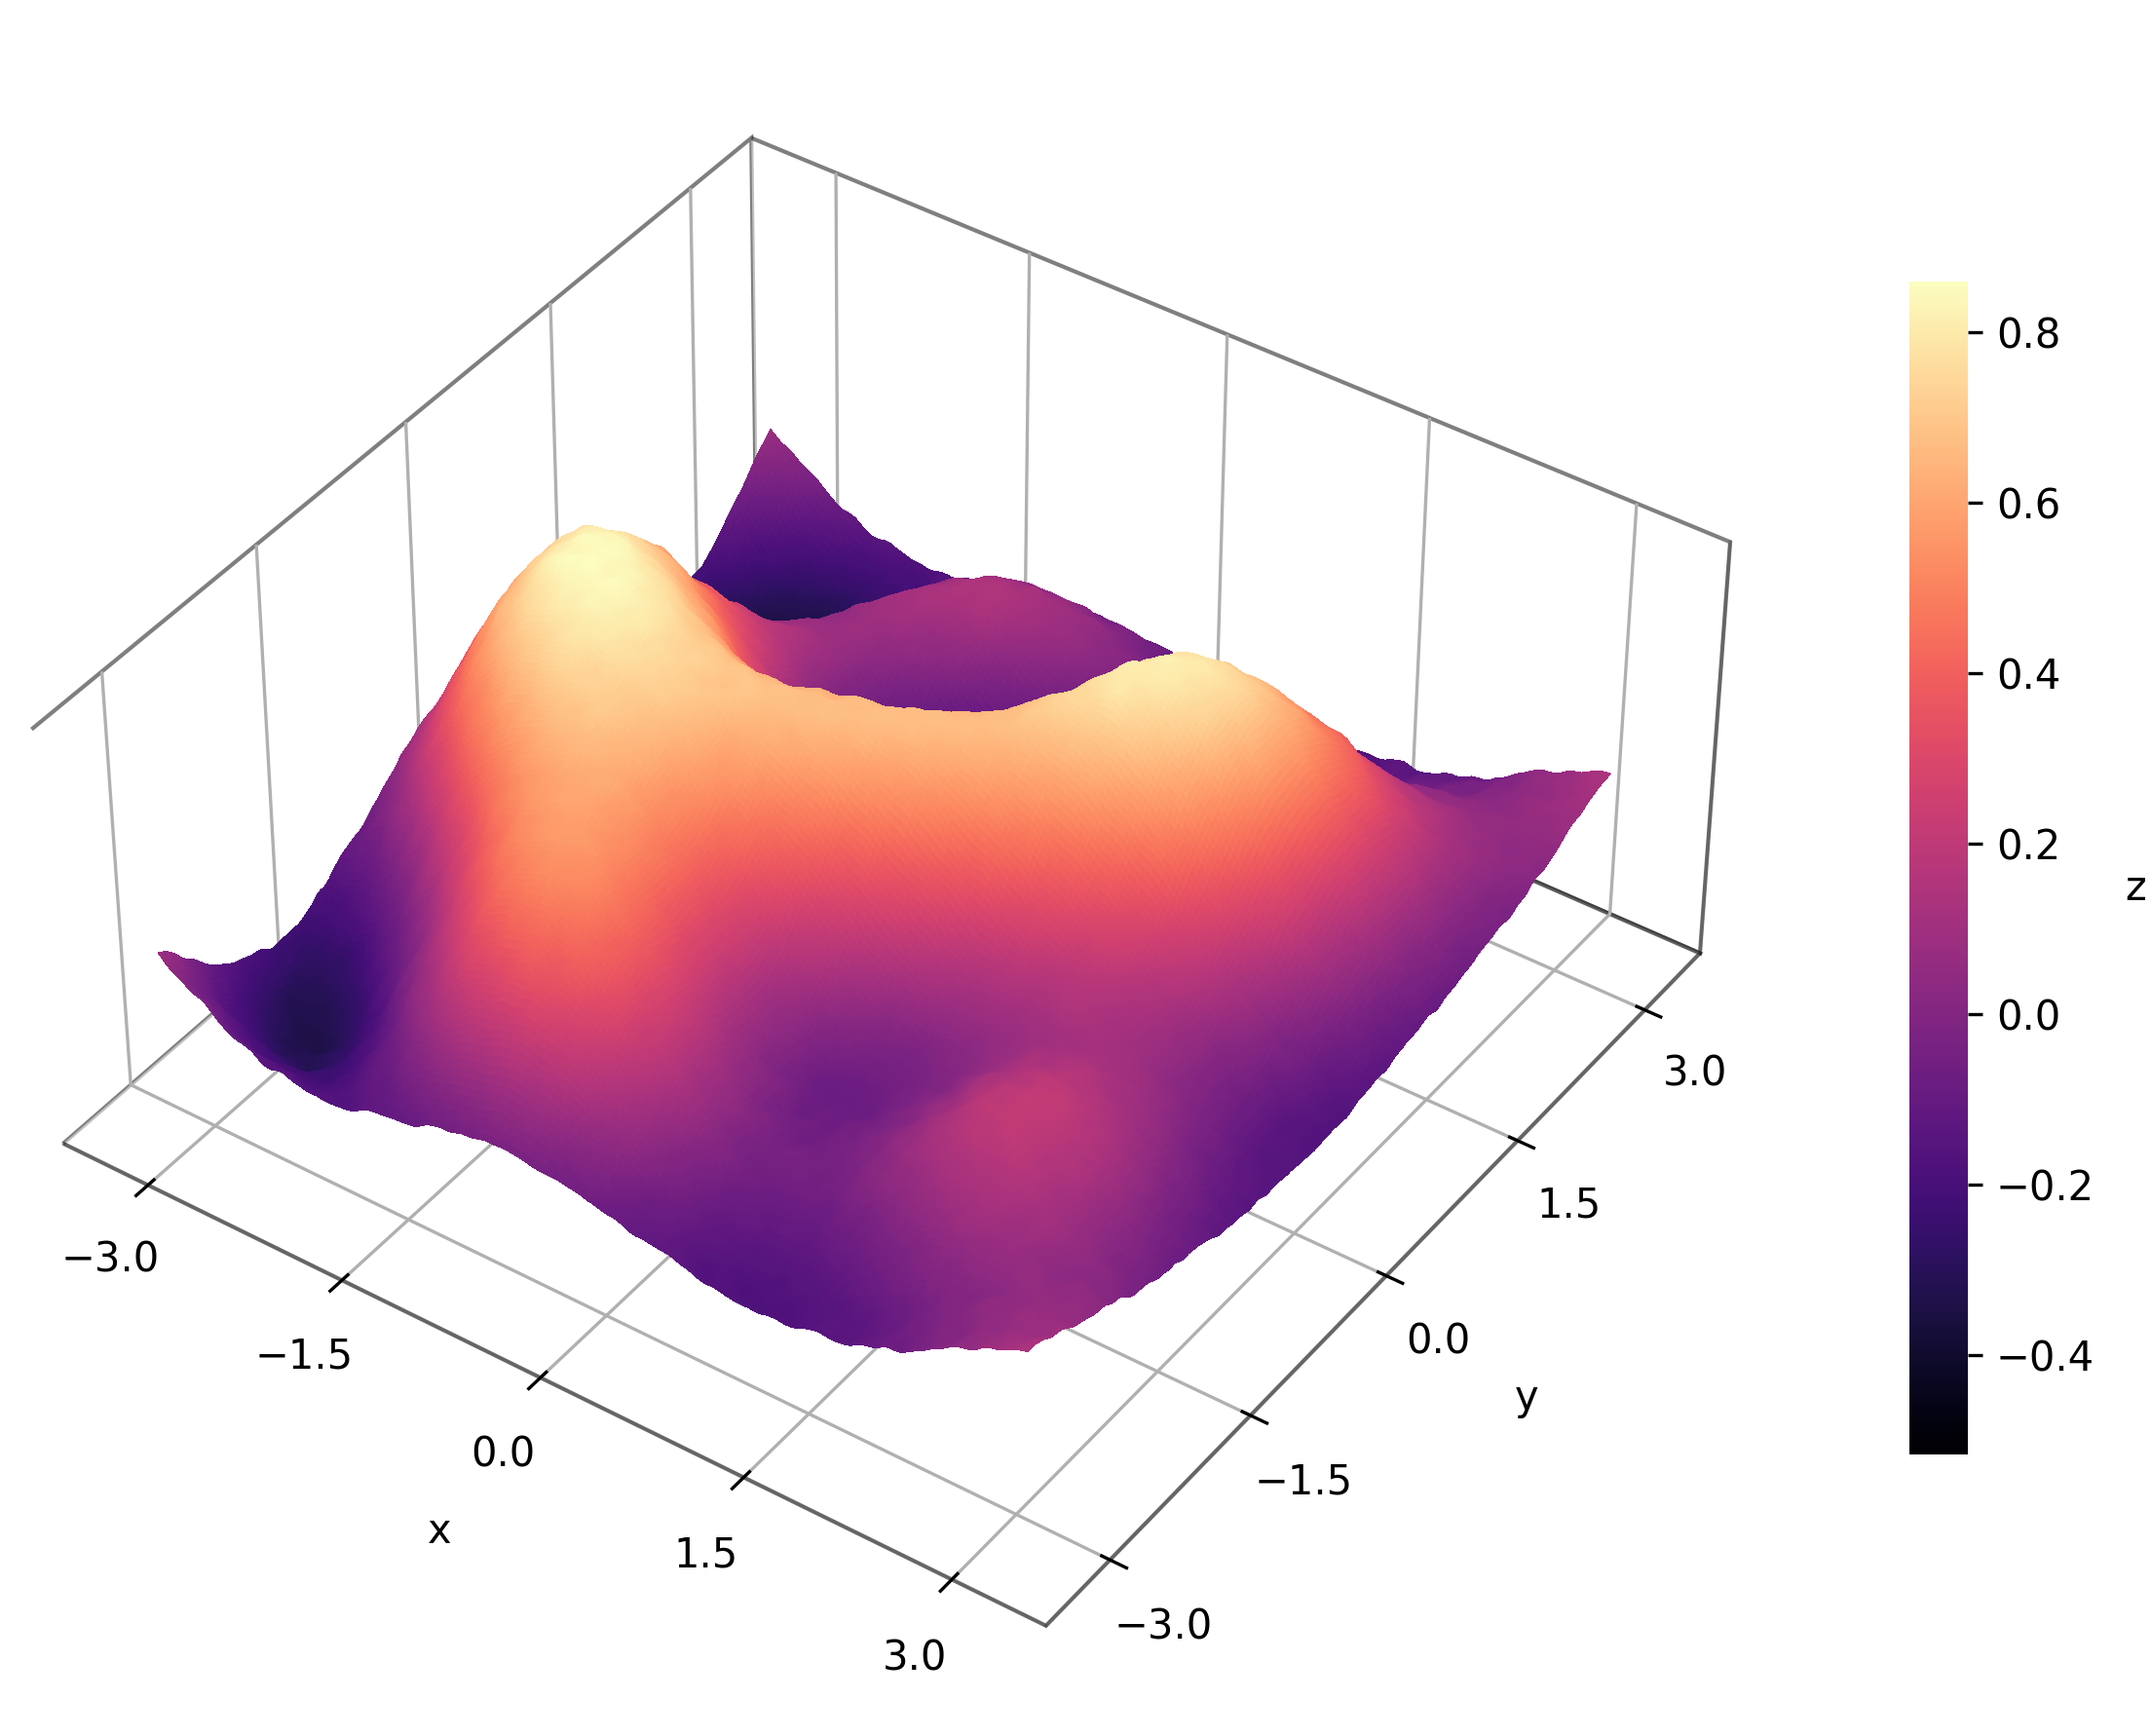
\includegraphics[width=0.5\linewidth]{figs/landscape.png}
	\end{figure}
\end{frame}

\begin{frame}{A Gaussian Process is a Distribution over Functions}
	\begin{columns}[T]
		\column{0.50\textwidth}
		\begin{itemize}[label=\textbullet]
			\setlength{\itemsep}{2.8em}
			\vspace{1.5em}
			\item A \textbf{multivariate Gaussian}: distribution over vectors.

			\item Depends on: the mean $\boldsymbol{\mu}$ vector and covariance matrix $\boldsymbol{\Sigma}$.
		\end{itemize}

		\column{0.49\textwidth}
		\begin{figure}
			\centering
			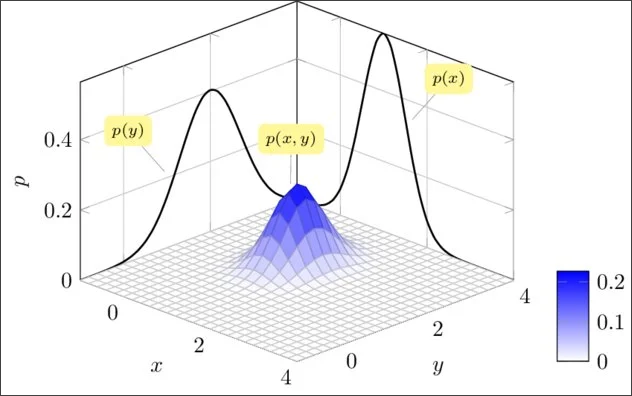
\includegraphics[
				width=0.99\linewidth,
				trim=4 4 4 4,
				clip
			]{figs/mulutivariable_normal2.png}
		\end{figure}
	\end{columns}

	\begin{itemize}[label=\textbullet]
	    \setlength{\itemsep}{1.8em}
	
		\item A \textbf{Gaussian Process ($\mathcal{GP}$)}: distribution over functions.
    	\[
			f(x) \sim \mathcal{GP}(m(x), k(x,x')).
    	\]

		\item Depends on: the mean function $m(x)$ and covariance function $k(x,x')$.
	\end{itemize}

	%\centering
	%\begin{tikzpicture}
	%
	%\node (img) at (0,0) {
	%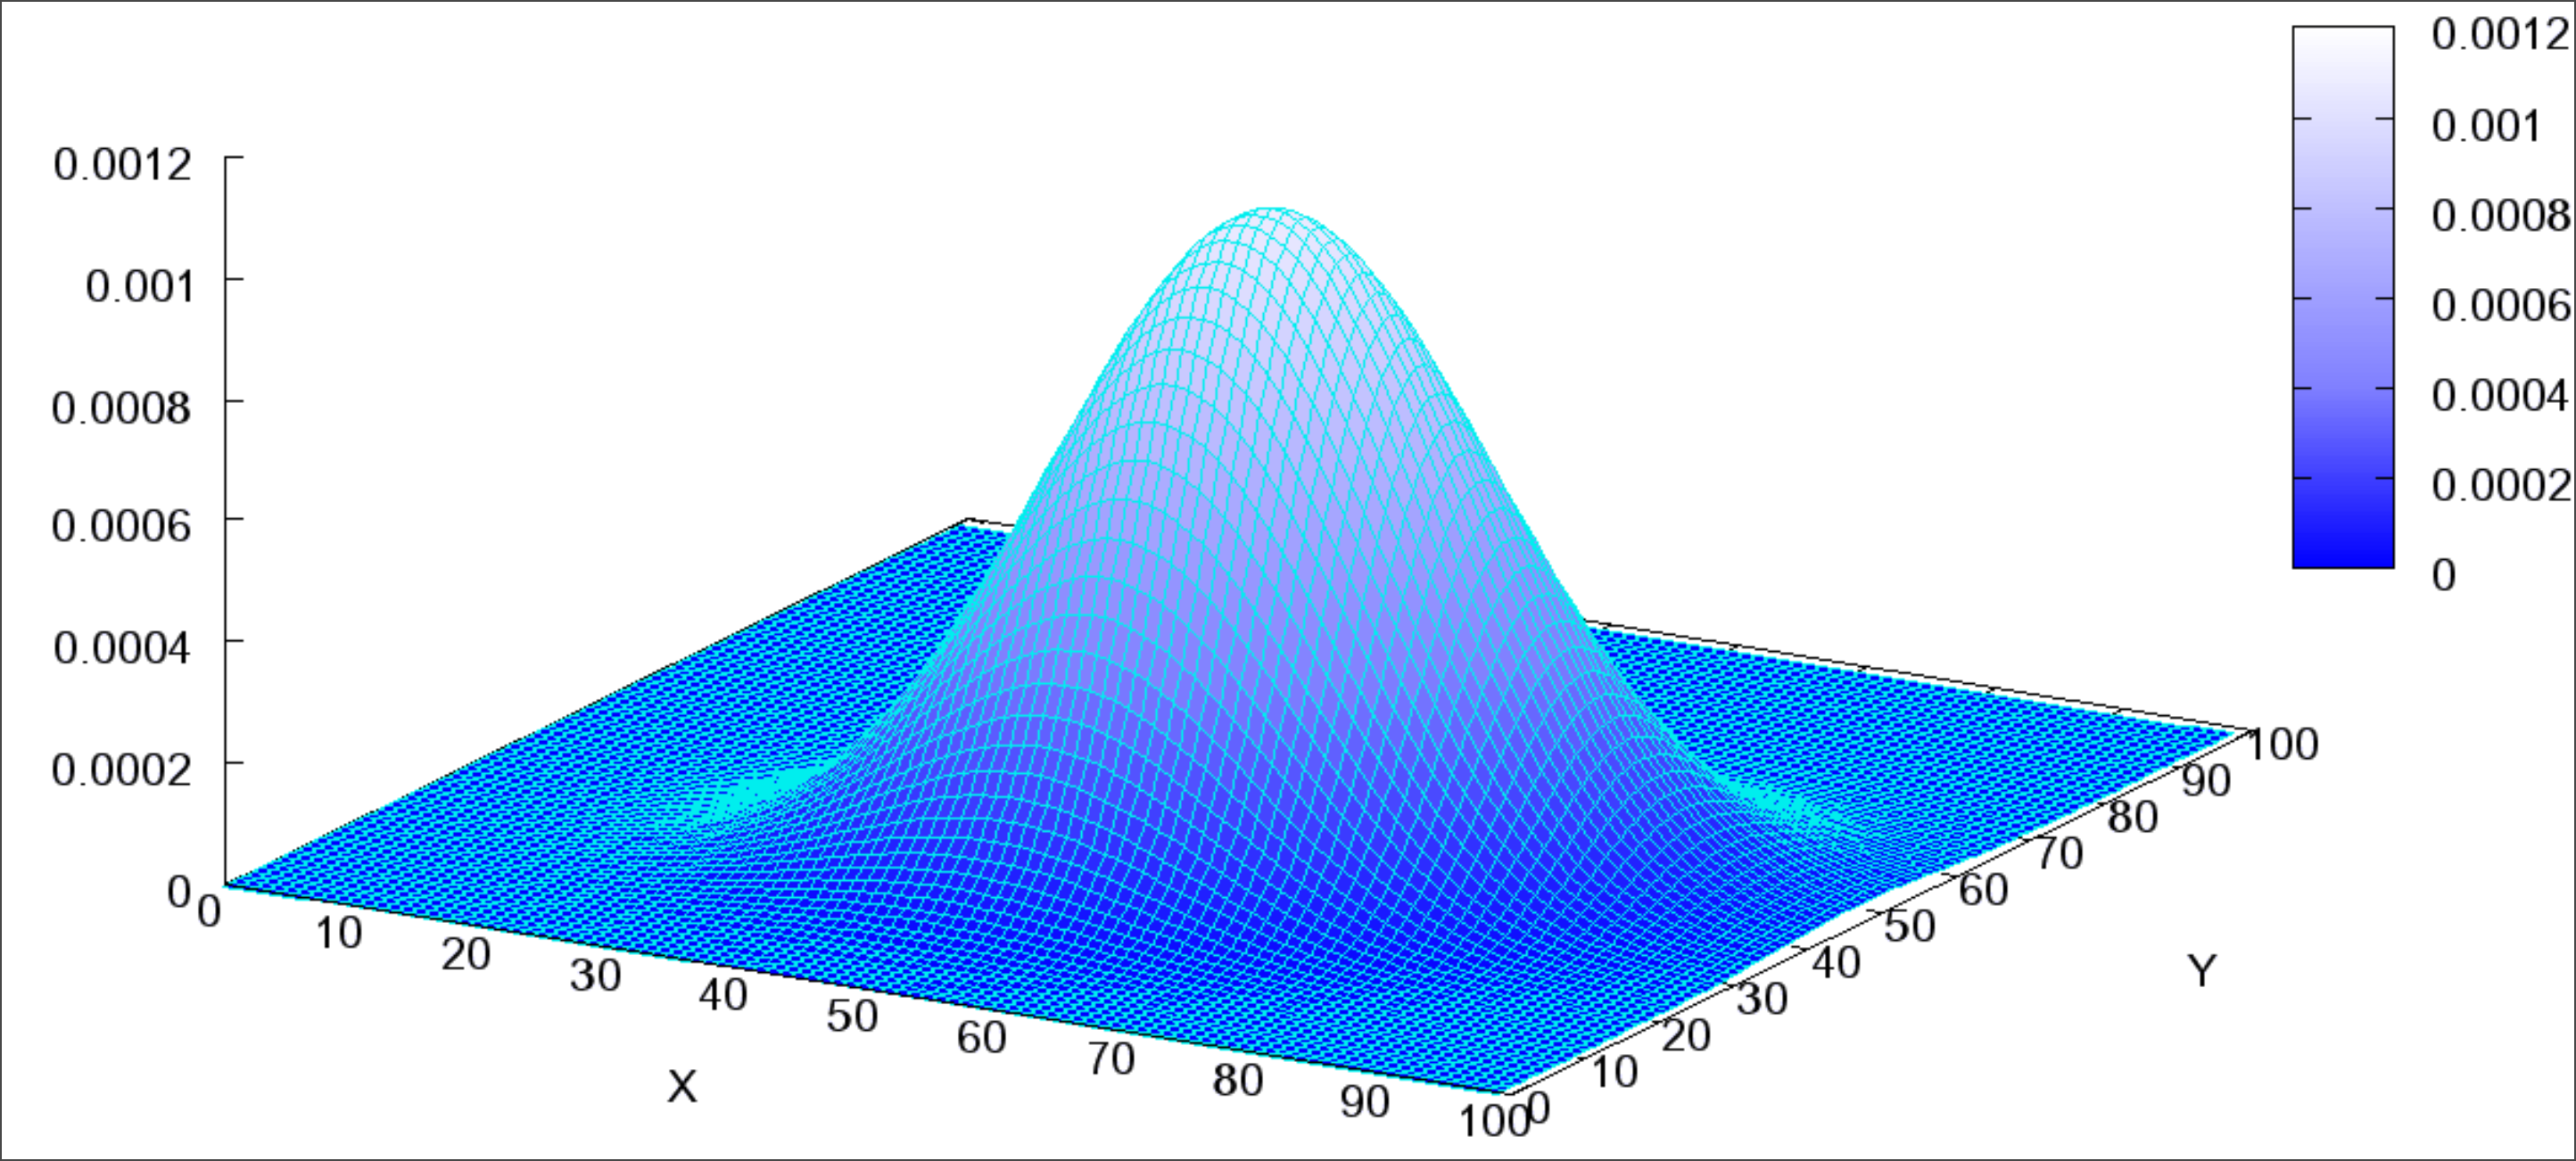
\includegraphics[
	%    width=0.4\textheight,
	%    trim=290 10 370 10,
	%    clip
	%]{figs/multivariate_normal.png}
	%};
	%
	%\node (arrow) at (3.0,0) {\Huge $\longrightarrow$};
	%
	%\node (inf) at (4.5,0) {\Huge $\infty$};
	%
	%\end{tikzpicture}
	\footnotetext{\tiny Image from: https://stackoverflow.com/questions/61291847/visualizing-a-multivariate-normal-distribution-in-3d-with-python}

\end{frame}


%\begin{frame}{Key Idea}
%\begin{itemize}
%    \setlength{\itemsep}{1.6em}
%	\item A \textbf{Gaussian Process (GP)} describes a distribution over functions.
%	\item $\quad\to\quad$Defined by a mean function $m(x)$ and covariance function $k(x,x')$.
%\end{itemize}
%
%\[
%	f(x) \sim \mathcal{GP}(m(x), k(x,x'))
%\]
%
%\[ 
%	m(x) = \mathbb{E}[f(x)] 
%	 = \int f(x) p(f) df
%\]
%\[
%	k(x,x') = \mathbb{E}[(f(x) - m(x))(f(x') - m(x'))]
%\]
%\[
%	 = \int (f(x) - m(x))(f(x') - m(x')) p(f) df
%\]
%
%\end{frame}

\begin{frame}{Gaussian Process Example}
	\begin{itemize}
		\setlength{\itemsep}{1em}
		\item $y(x) \sim \mathcal{GP}\bigl(m(x), k(x, x')\bigr)$ gives us the \textbf{mean} and \textbf{uncertainty}.\\
		\item \textbf{Key Idea}: Sampling $(y(x_1), y(x_2), \ldots)$ gives a multivariate Gaussian.
	\end{itemize}
	\begin{figure}
		\centering
		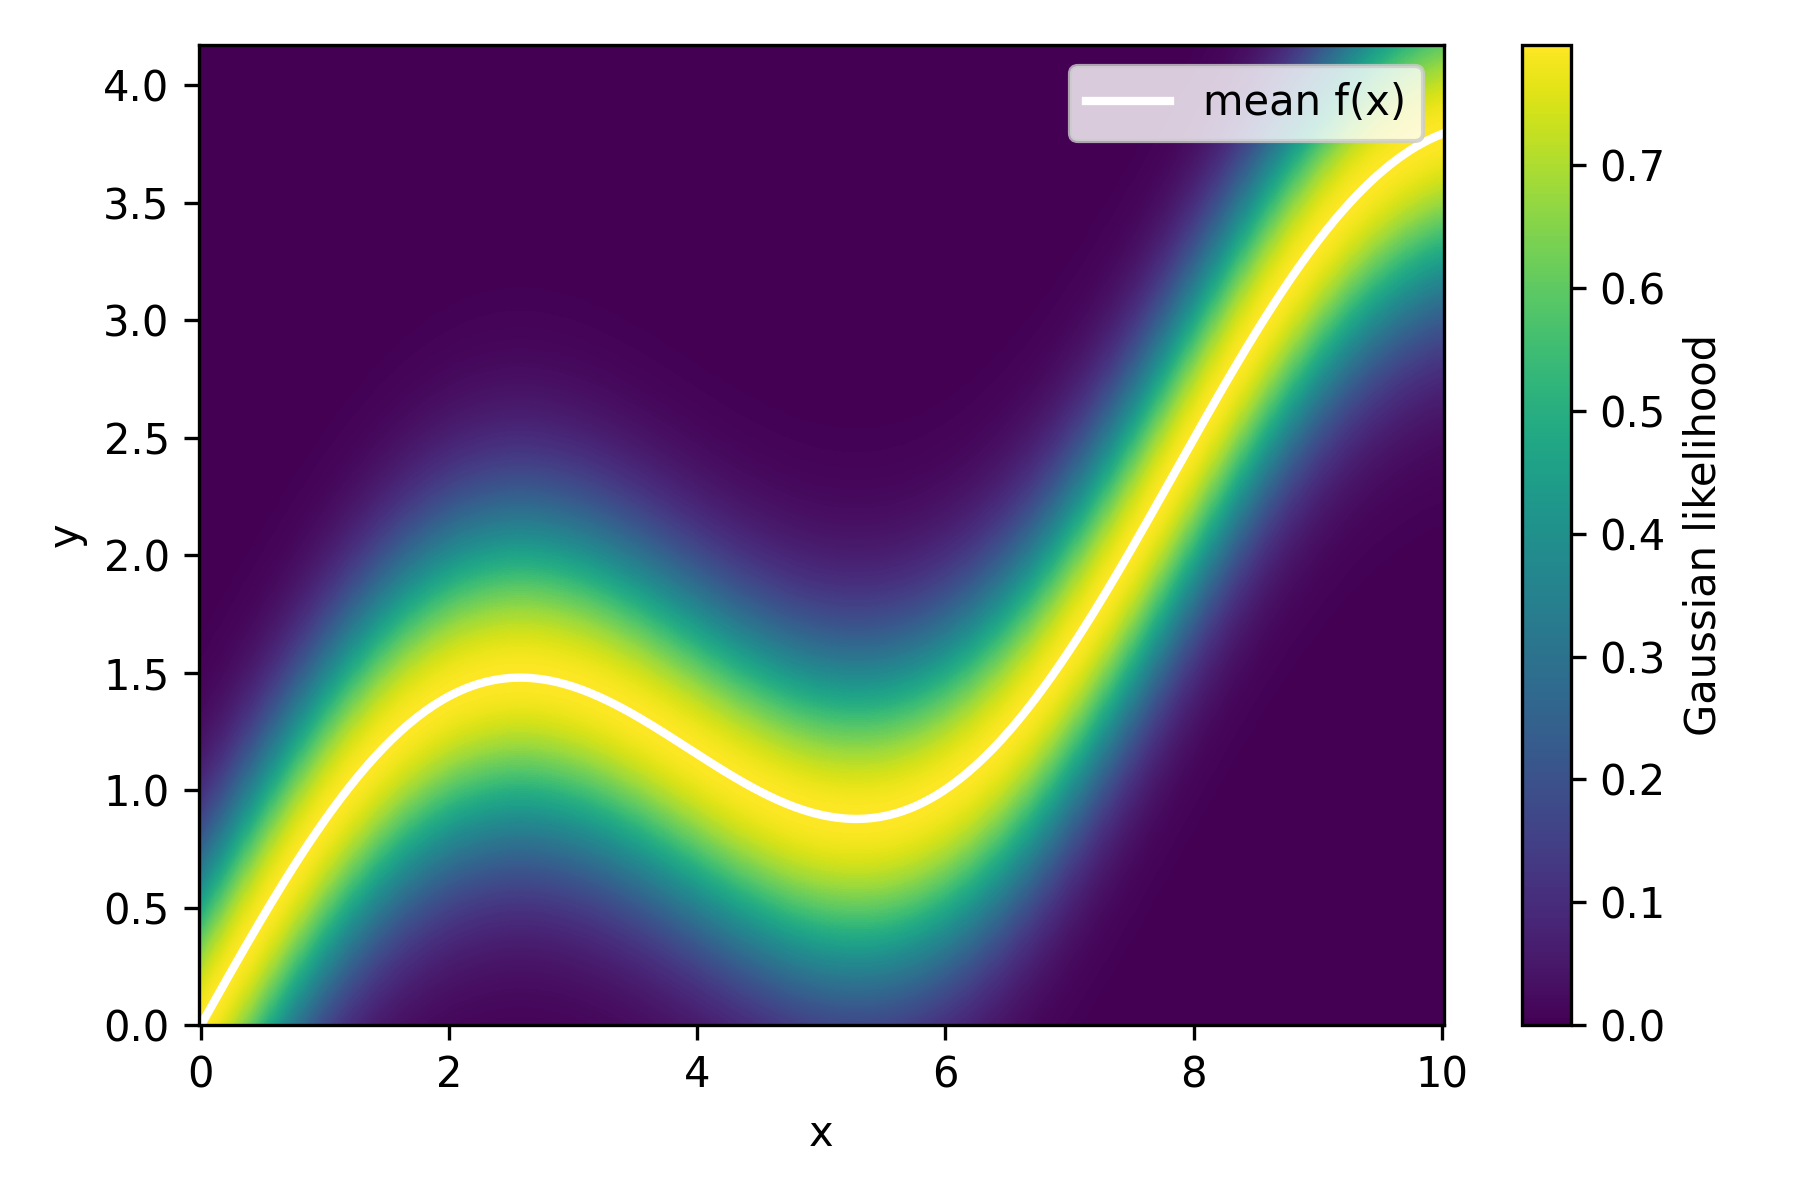
\includegraphics[
			width=0.75\linewidth,
			trim=2 2 2 2,
			clip
		]{figs/example_GP_plot.png}
	\end{figure}
\end{frame}

\begin{frame}{Bayesian Linear Regression}
	
	% --- Top row ---
	\begin{columns}[T]
	\column{0.55\textwidth}
	
	\textbf{Model assumptions:}
	\vspace{1.0em}
	
	\begin{itemize}
	\setlength{\itemsep}{1.5em}
	
	\item Linear model:
	\(
	f(\mathbf{x}) = \sum_{j=1}^d w_j x_j.
	\)
	
	\item Gaussian prior:
	\(
	\mathbf{w} \sim \mathcal{N}(\mathbf{0}, \sigma_w^2 I).
	\)
	
	\item Gaussian noise:
	\(
	y = f(\mathbf{x}) + \varepsilon.
	\)

	\item \textbf{Bayes' theorem} $\implies$ the posterior over weights is Gaussian:
	\[
		p(\mathbf{w}\mid X,\mathbf{y}) = \frac{p(\mathbf{y}\mid X,\mathbf{w})\,p(\mathbf{w})}{p(\mathbf{y}\mid X)}.
	\]

	\item Can use $p(\mathbf{w}\mid X,\mathbf{y})$ to make predictions at new inputs $\mathbf{x}_*$ but there is a better way!

	\end{itemize}
	
	\column{0.45\textwidth}
	\centering
	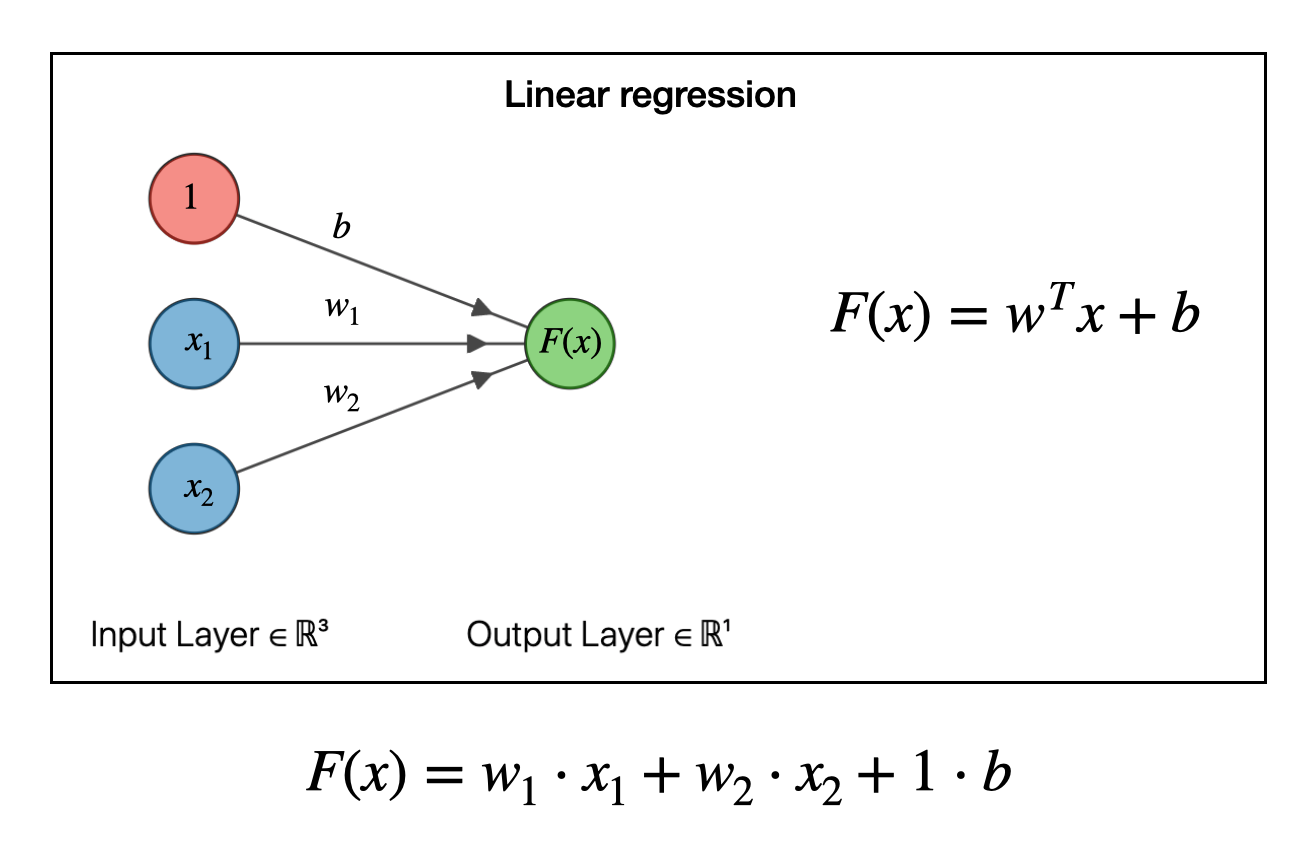
\includegraphics[
	width=0.9\linewidth,
	trim=100 300 500 150,
	clip
	]{figs/linear_regression.png}
	{\tiny https://joshuagoings.com/2020/05/05/neural-network/}

	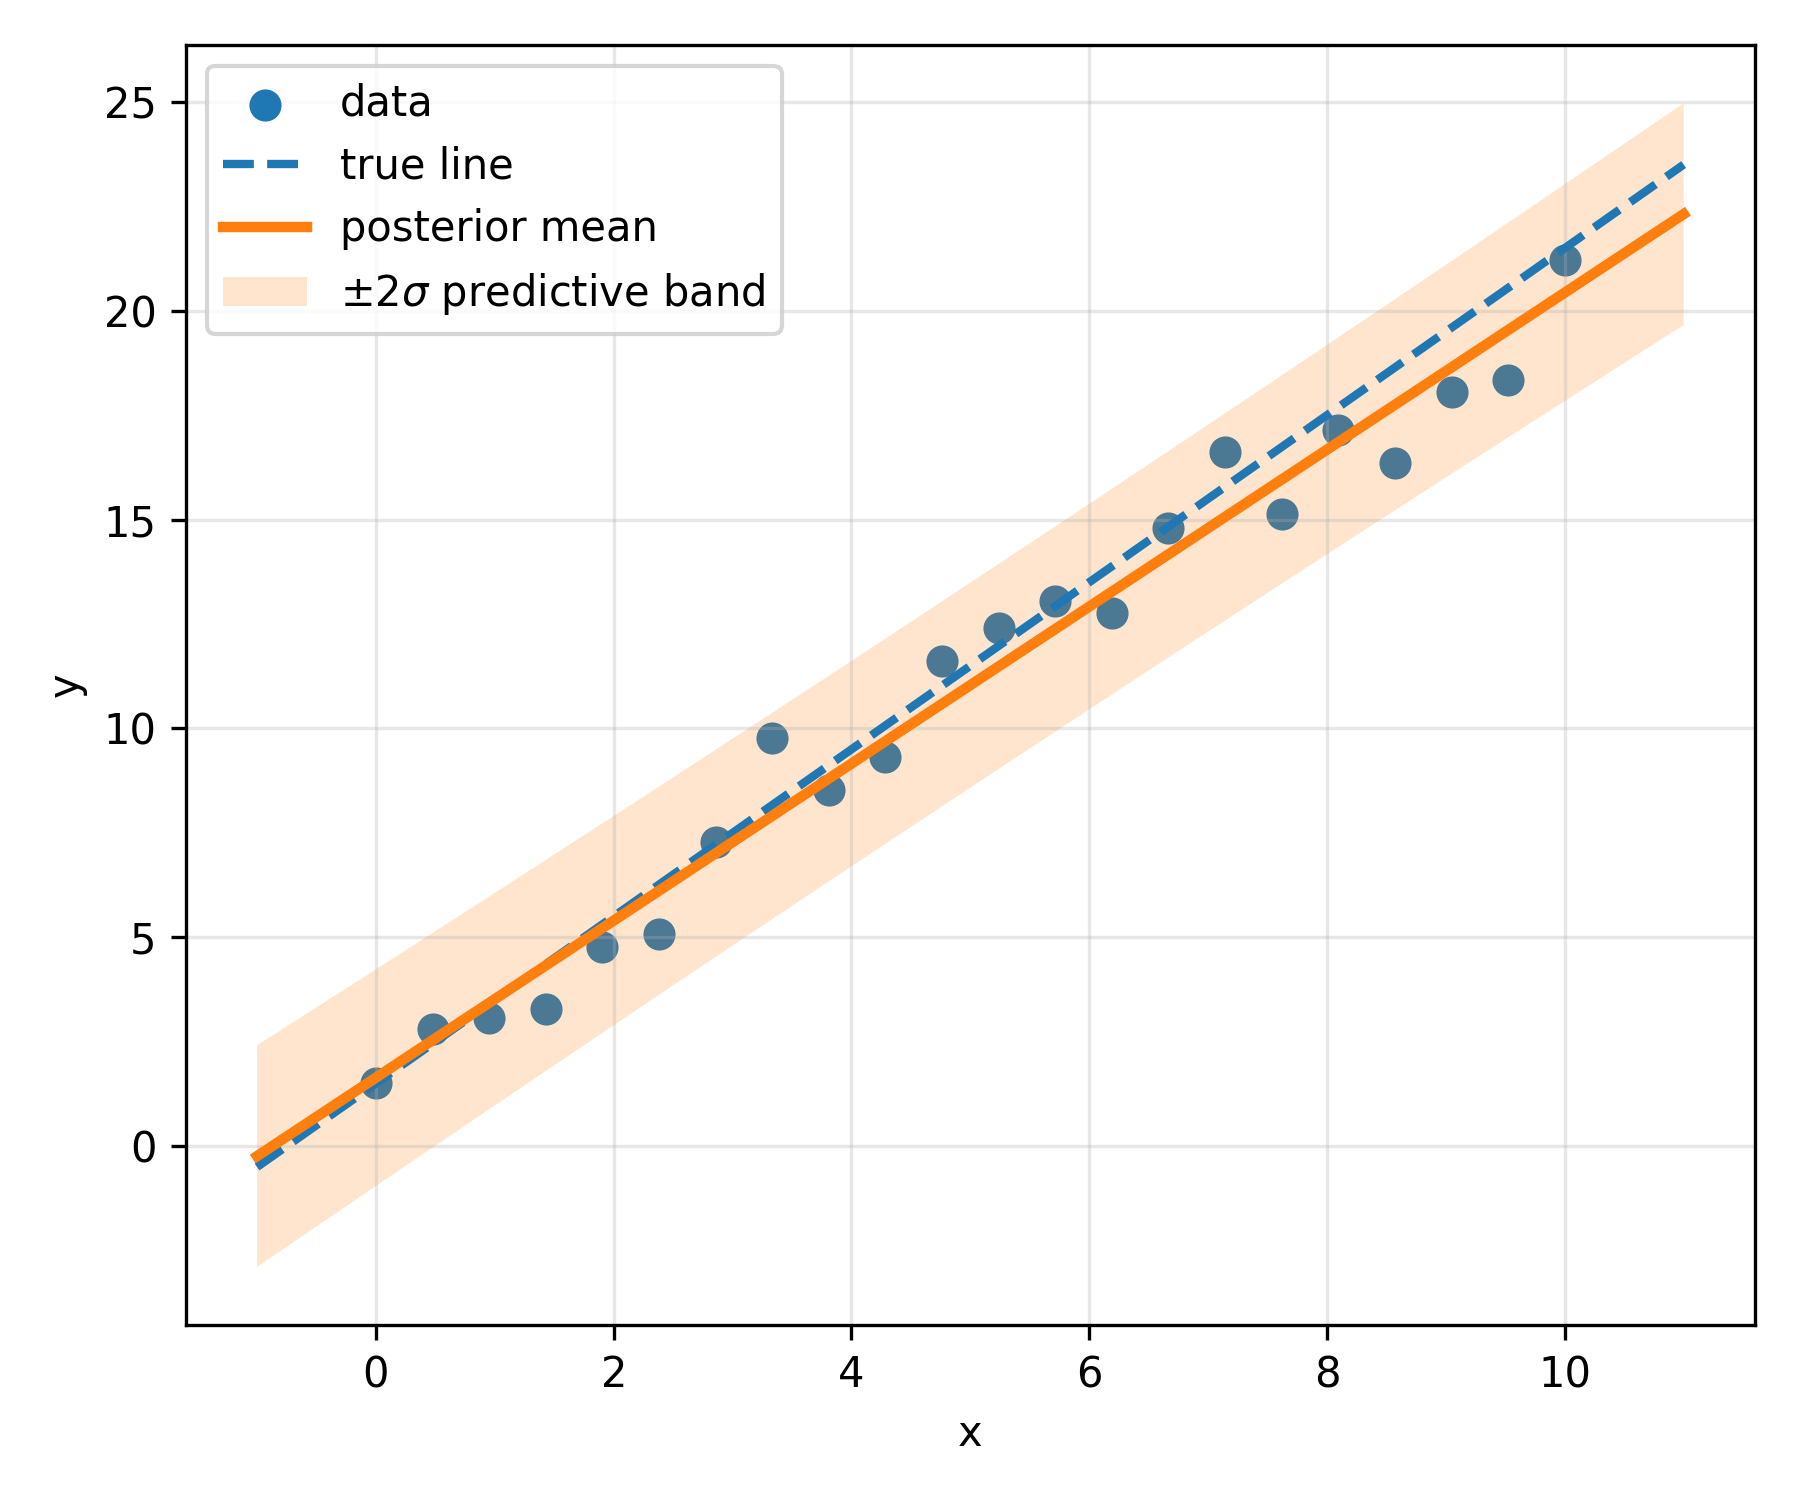
\includegraphics[width=0.9\linewidth, trim=1 1 1 1, clip]{figs/bayesian_lin_reg.png}
	
	\end{columns}
	
	\vspace{0.6em}
	
	%\begin{itemize}
	%\setlength{\itemsep}{0.7em}

	%\vspace{1.5em}
	%
	%\item \textbf{Bayes' theorem} $\implies$ the posterior over weights is Gaussian:
	%\[
	%p(\mathbf{w}\mid X,\mathbf{y})
	%\propto
	%p(\mathbf{y}\mid X,\mathbf{w})\,p(\mathbf{w})
	%\]
	%
	%%\item Gaussian prior + Gaussian likelihood
	%%$\Rightarrow$
	%%\[
	%%p(\mathbf{w}\mid X,\mathbf{y})
	%%=
	%%\mathcal{N}(\boldsymbol{\mu}_w,\boldsymbol{\Sigma}_w)
	%%\]
	%
	%\item Predictive distribution of $f_*$ at a new input $\mathbf{x}_*$ is Gaussian:
	%	\[
	%	p(f_*\mid \mathbf{x}_*,X,\mathbf{y})
	%	=
	%	\int p(f_* \mid \mathbf{x}_*,\mathbf{w})\,p(\mathbf{w}\mid X,\mathbf{y})\,d\mathbf{w}
	%	=
	%	\mathcal{N}(\mu_*,\sigma_*^2)
	%	\]
	%	and does \textbf{not} depend on $\mathbf{w}$.
	%\end{itemize}

\end{frame}


\begin{frame}{From Linear Models to Infinite Feature Spaces}

	\begin{columns}[T]
	
	\column{0.54\textwidth}
	\begin{itemize}
	\setlength{\itemsep}{1.6em}

	\item \textbf{Problem:} Linear models are too simple.
	
	\item \textbf{Solution:} introduce a feature map:
	\[
	f(\mathbf{x}) = \boldsymbol{\phi}(\mathbf{x})^\top \mathbf{w}.
	\]

	\item Example: polynomial feature map
	\[
		\boldsymbol{\phi}(\mathbf{x}) = (1, x, x^2, \ldots)^\top \in \mathbb{R}^D.
	\]

	\item $D \to \infty$ to capture all possible functions.
	
	\end{itemize}
	
	\column{0.45\textwidth}
	\begin{figure}
	\centering
	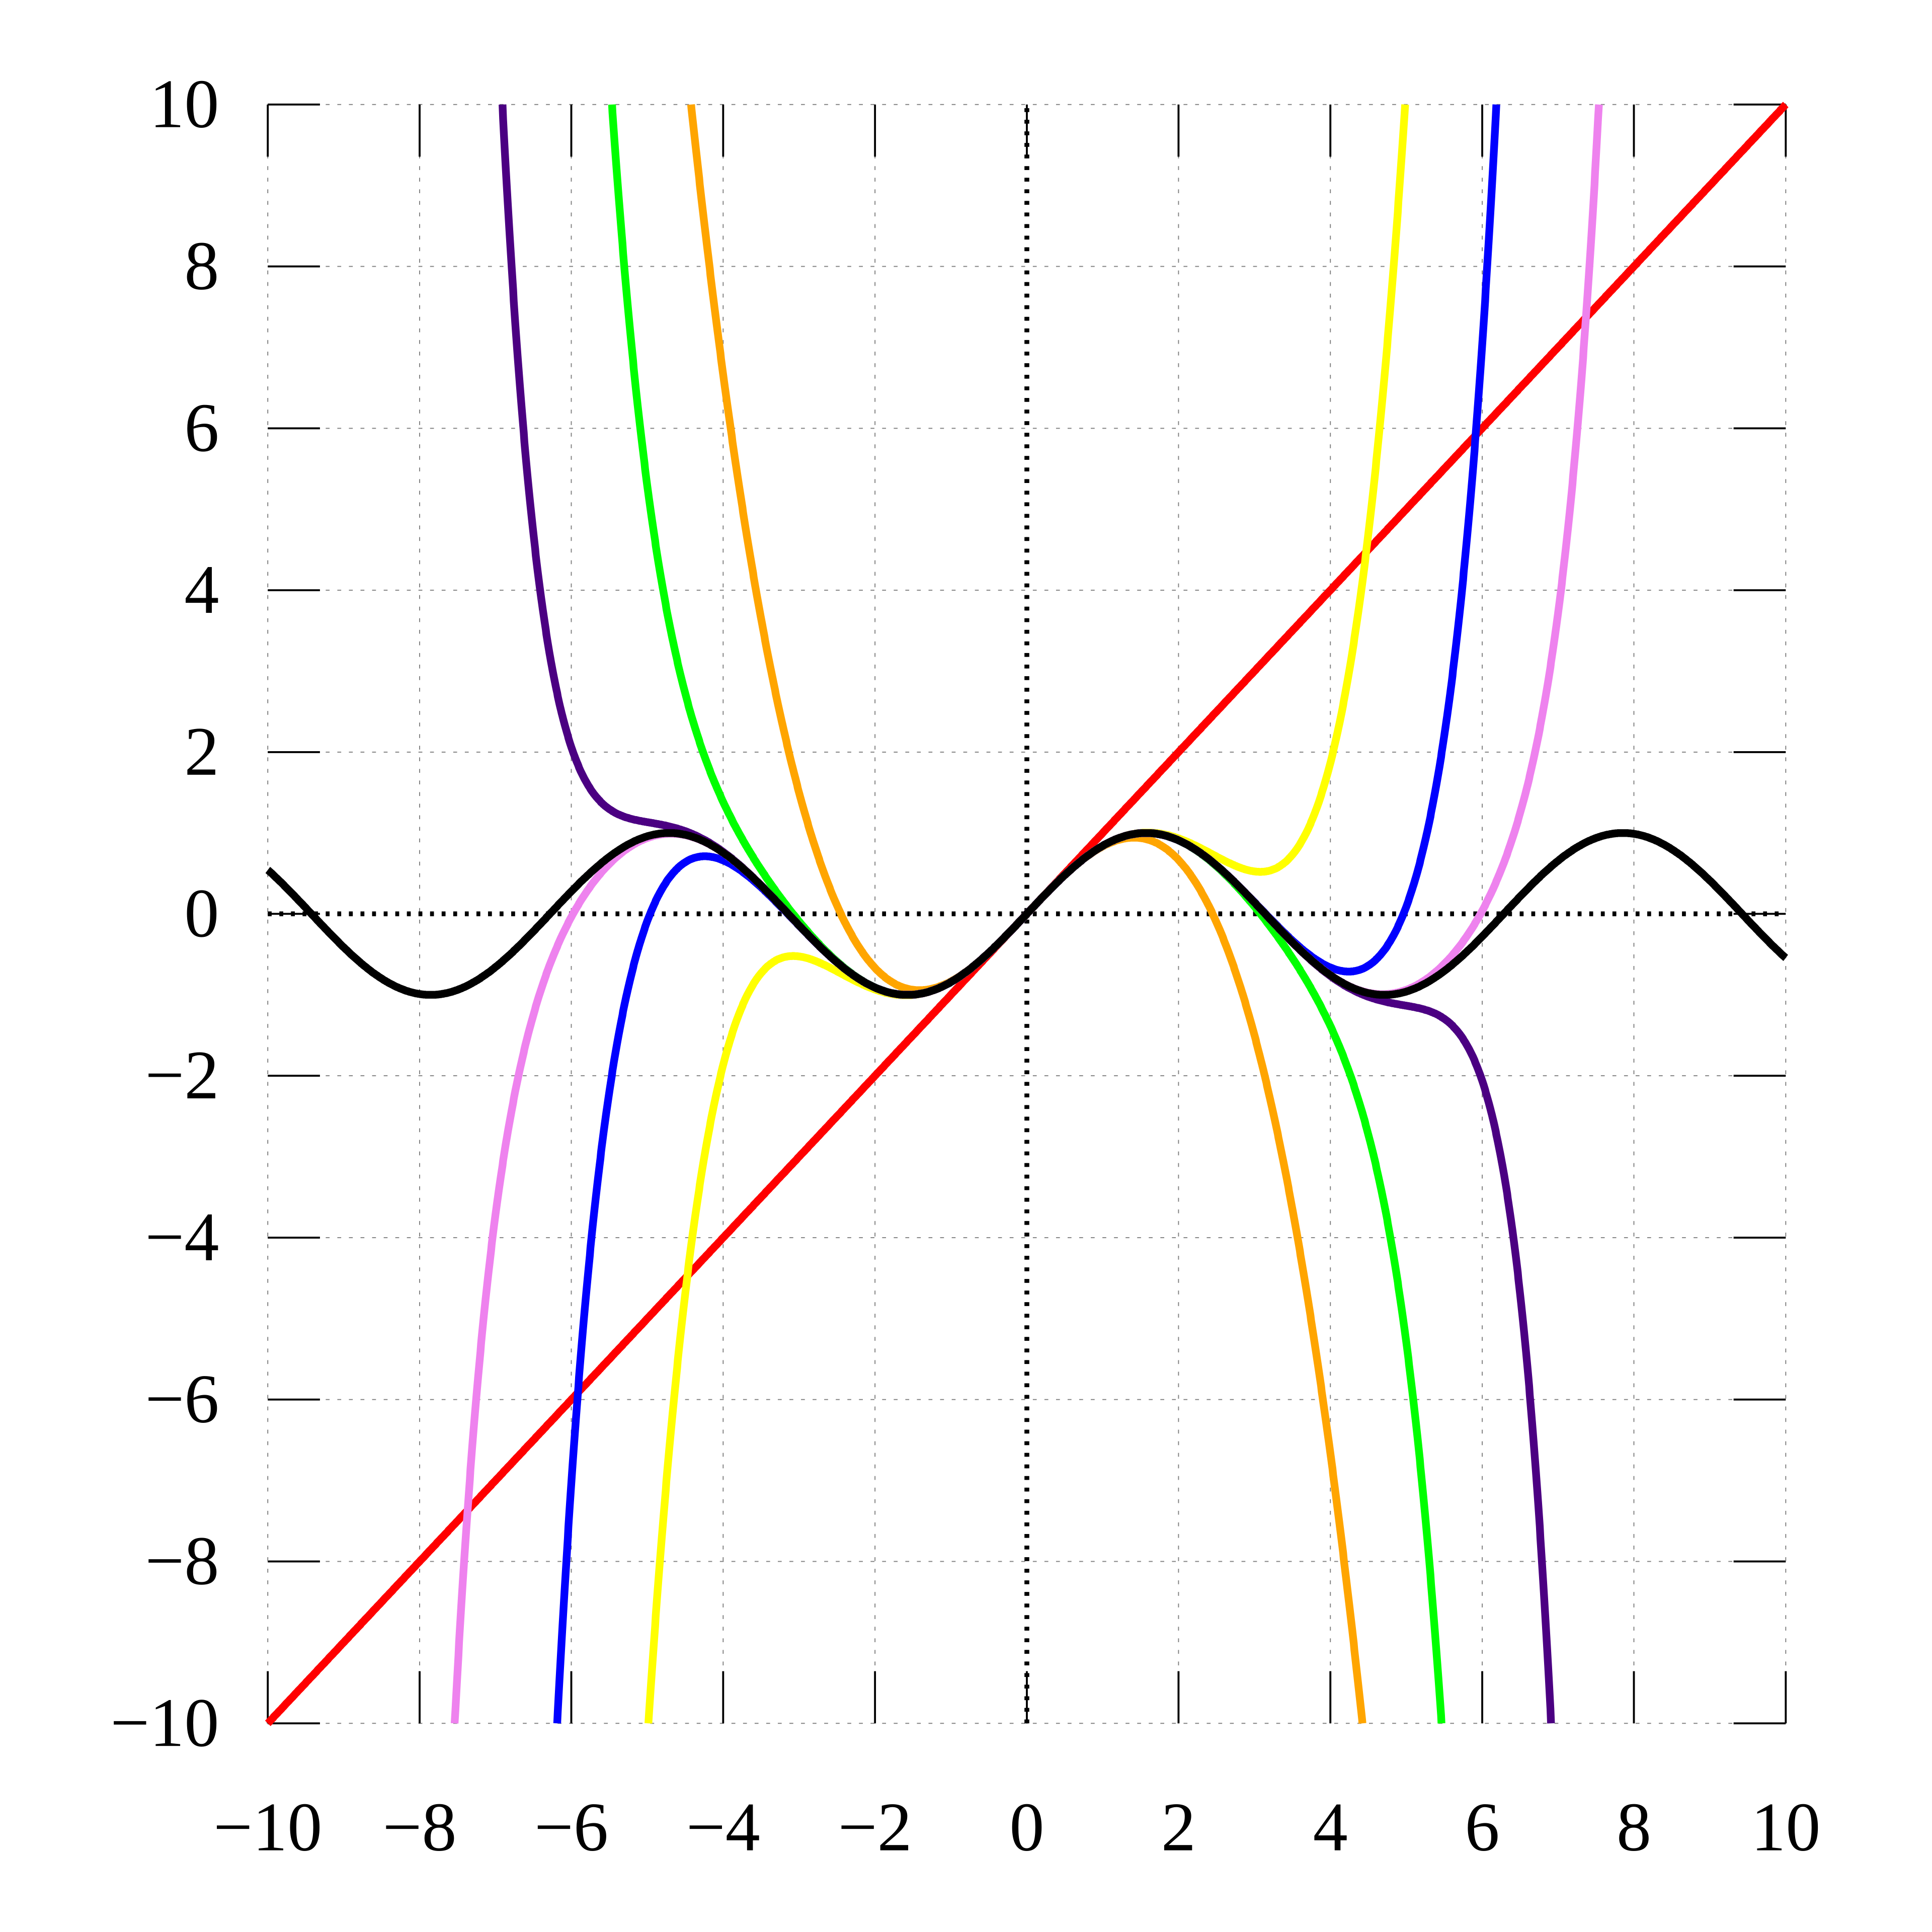
\includegraphics[
	width = 0.9\linewidth,
	trim=4 4 4 4,
	clip
	]{figs/taylor.png}
	\end{figure}
	
	\end{columns}
	
	\vspace{1em}
	
	\begin{itemize}
	\setlength{\itemsep}{1.5em}
	
	\item \textbf{New Problem:} If we want to model all functions we need an infinite number of parameters (weights).
	\end{itemize}
\end{frame}


\begin{frame}{Infinite Features via the Kernel Trick}
	\begin{itemize}[label=\textbullet]
	\setlength{\itemsep}{1.4em}
	
	\item Guassian process defined by:
	\[
	m(x) = \mathbb{E}[f(x)], \qquad
	k(x,x') = \mathbb{E}[f(x)f(x')].
	\]
	
	\item For a linear model with features $\boldsymbol{\phi}(x)$ and 
	$\mathbf{w} \sim \mathcal{N}(0, \sigma_w^2 I)$:
	\[
	m(x) = 0, \qquad
	k(x,x') = \sigma_w^2 \, \boldsymbol{\phi}(x)^\top \boldsymbol{\phi}(x').
	\]
	
	\item Example feature map:
	\[
	\boldsymbol{\phi}(x) = \left(1, x, \tfrac{x^2}{\sqrt{2!}}, \tfrac{x^3}{\sqrt{3!}}, \dots \right)
	\]
	
	\item Inner product becomes:
	\[
	k(x,x') = \sum_{n=0}^{\infty} \frac{(x x')^n}{n!} = e^{x x'}.
	\]
	
	\item \textbf{Key idea:} compute kernels directly $\Rightarrow$ implicit infinite features.
	
	\end{itemize}
\end{frame}

\begin{frame}{Gaussian Process Regression}
	\begin{itemize}
	\setlength{\itemsep}{1.4em}
	%\item By definition of a $\mathcal{GP}$, the joint distribution of observed data and a new point $x_*$ is also Gaussian:
	\item Sampling a $\mathcal{GP}$ at \red{X} and a new point \blue{$\mathbf{x}_*$} gives a \textbf{joint Gaussian}:
	\begin{figure}
		\centering
		% Example of a two single variable gaussian distributions with a joint distribution between them.
		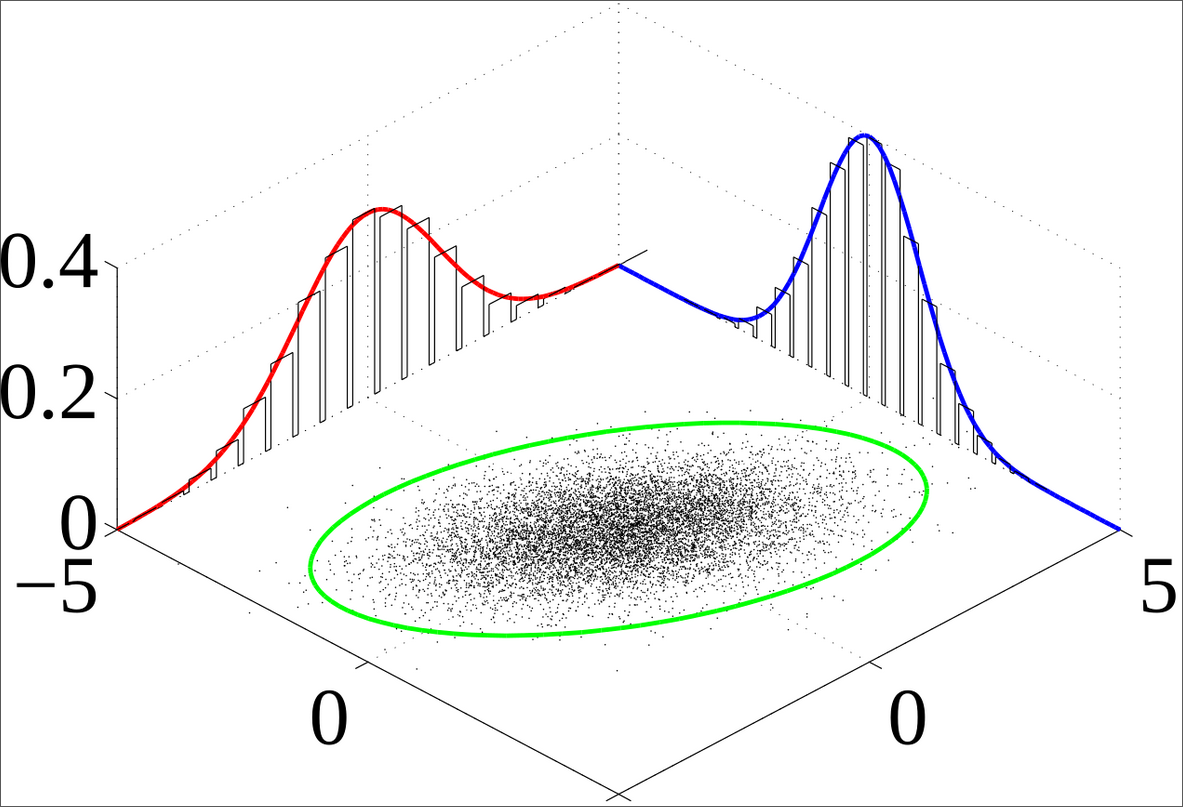
\includegraphics[width=0.4\linewidth, trim=4 4 4 6, clip]{figs/joint_gaussian.png}
		\footnote{\tiny https://en.wikipedia.org/wiki/Multivariate\_normal\_distribution}
	\end{figure}
	\item \red{Red:} $\mathbf{y} \sim \mathcal{N}(\mathbf{0}, k(\mathbf{x}_i,\mathbf{x}_j))$ -- Prior distribution over observed data.
	\item \blue{Blue:} $f(\mathbf{x}_*) \sim \mathcal{N}(0, k(\mathbf{x}_*,\mathbf{x}_*))$ -- Prior distribution over new point.
	\item \green{Green:} $p(f(\mathbf{x}_*), \mathbf{y})$ -- Joint Gaussian distribution.
	\item \textbf{Final Result:} The conditional distribution:
	\[
		p(f(\mathbf{x}_*) \mid \mathbf{x}_*, X,\mathbf{y}) = \mathcal{N}(\mu_*,\sigma_*^2).
	\]
	\end{itemize}
\end{frame}

\begin{frame}{Summary of Gaussian Process Regression}
	\begin{figure}
		\centering
		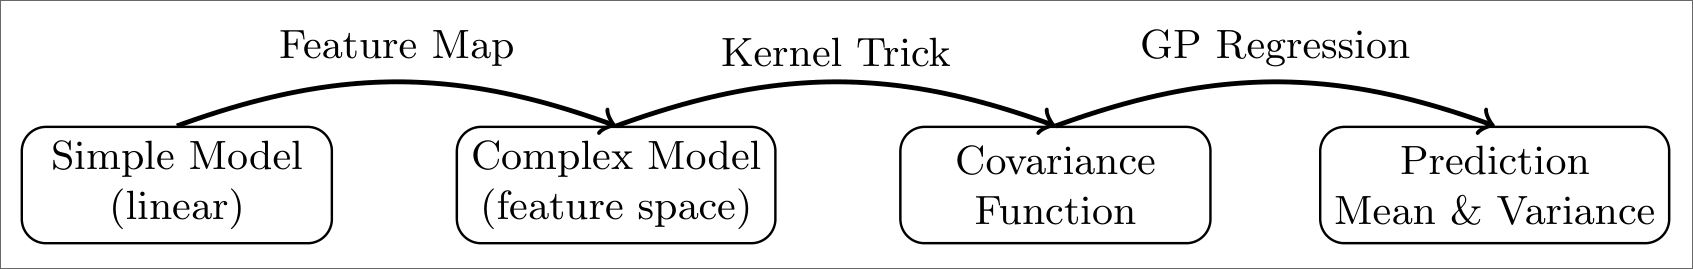
\includegraphics[height=0.19\textheight, trim=4 4 4 4, clip]{figs/GPR_diagram.png}
		%\begin{tikzpicture}[
		%scale=0.75,
		%transform shape,
		%node distance=3.4cm,
		%box/.style={draw, rounded corners, align=center, minimum width=2.4cm, minimum height=0.9cm},
		%arrow/.style={->, thick}
		%]
		%
		%\node[box] (simple) {Simple Model\\(linear)};
		%\node[box] (feature) [right of=simple] {Complex Model\\(feature space)};
		%\node[box] (kernel) [right of=feature] {Covariance\\Function};
		%\node[box] (result) [right of=kernel] {Prediction\\Mean \& Variance};
		%
		%\draw[arrow] (simple.north) to[bend left=20] node[above]{Feature Map} (feature.north);
		%\draw[arrow] (feature.north) to[bend left=20] node[above]{Kernel Trick} (kernel.north);
		%\draw[arrow] (kernel.north) to[bend left=20] node[above]{GP Regression} (result.north);
		%
		%\end{tikzpicture}
	\end{figure}
	%\vspace{-1em}
	\begin{figure}
		\centering
		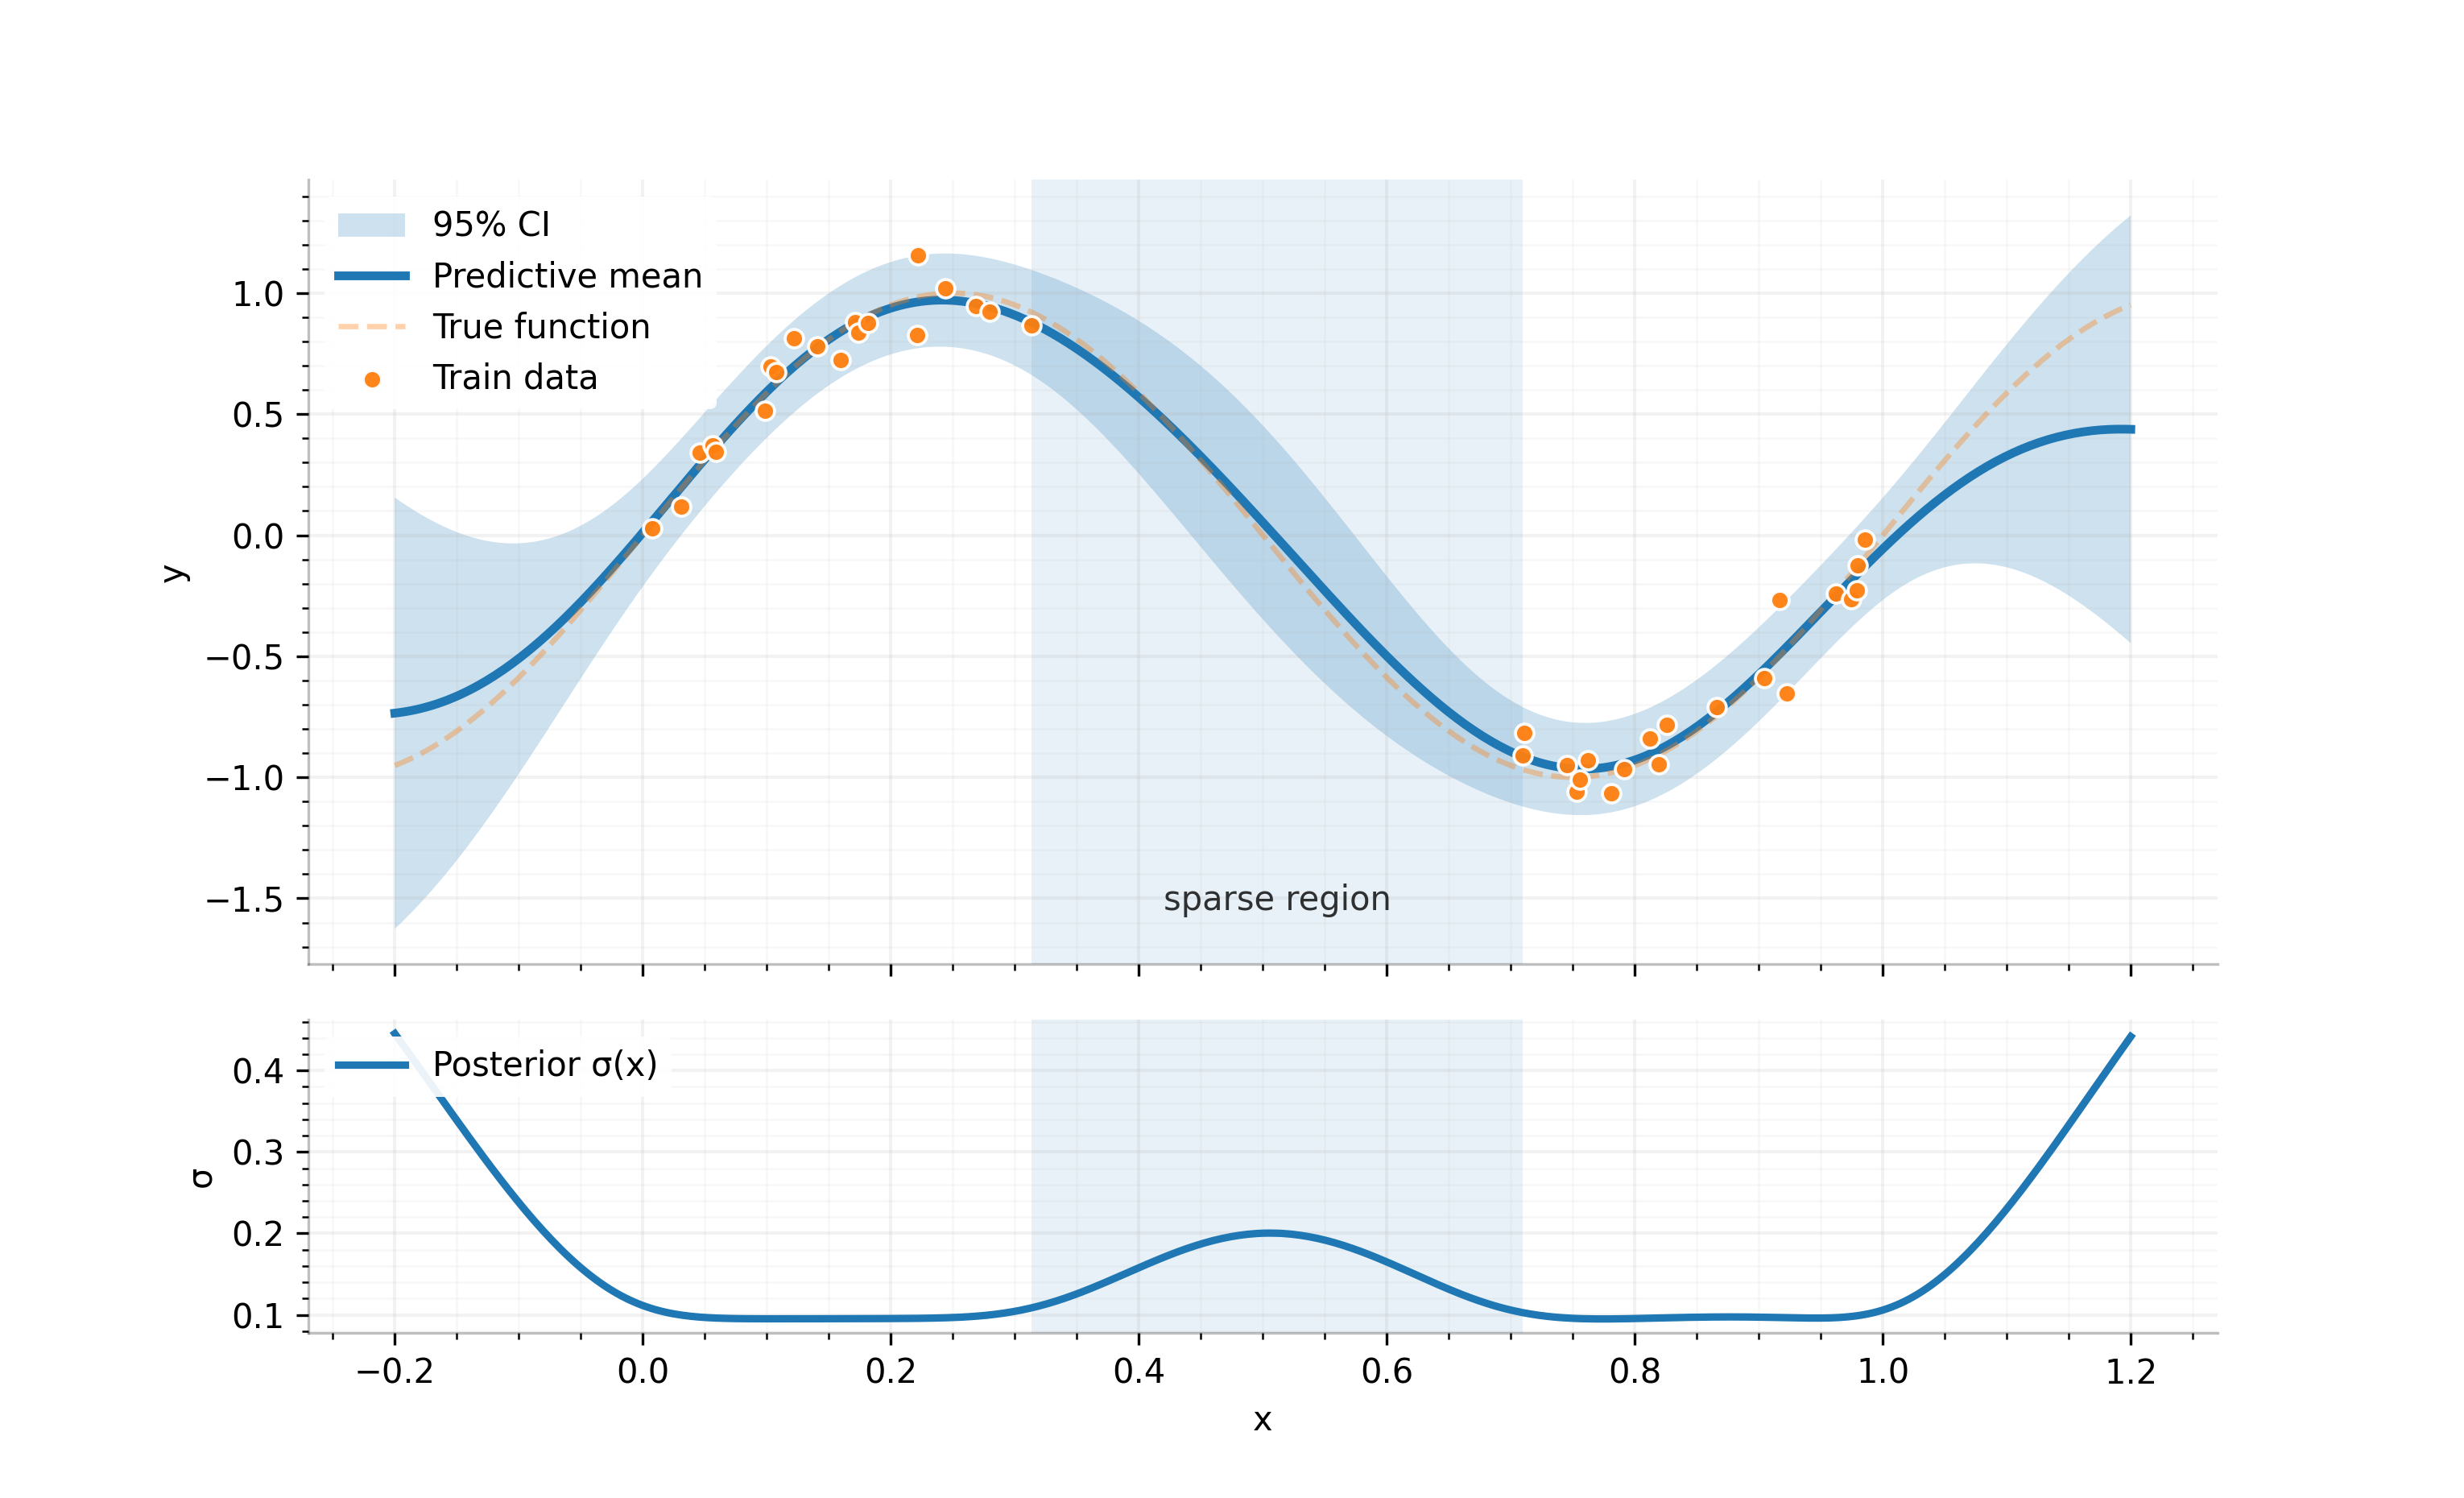
\includegraphics[height=0.60\textheight, trim=0 0 0 50, clip]{figs/gpr_gptorch.png}
		% Plot showing data points samples from a sin(x) function. 
		% Data on left and right but not in middle 
		% Variance increases in middle where there is no data
	\end{figure}
\end{frame}


\begin{frame}{The Acquisition Function}
	\begin{figure}
		\centering
		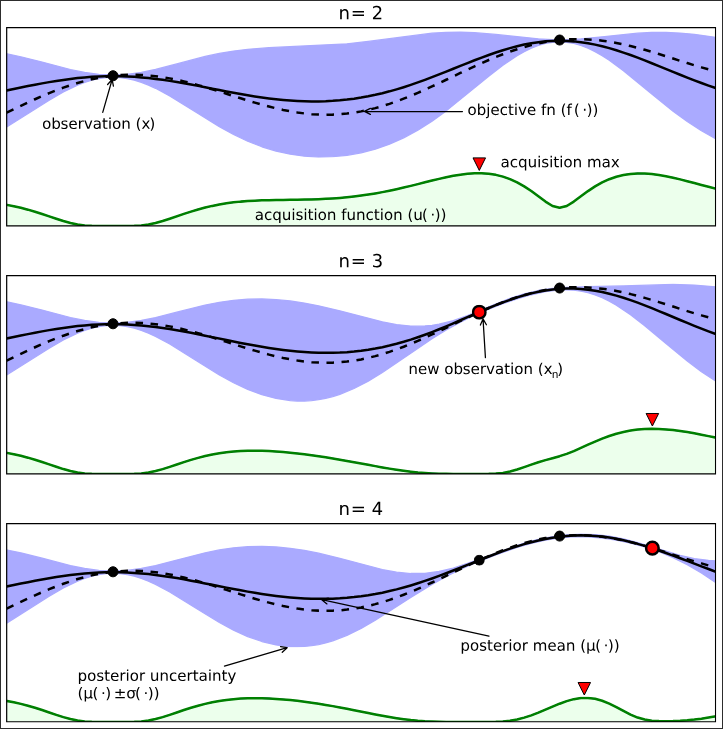
\includegraphics[height=0.8\textheight, trim = {4 4 4 4}, clip]{figs/active_learning_example1.png}
			\footnote{
				\tiny
				Shahriari, B., et al. (2016). Taking the Human Out of the Loop: A Review of Bayesian Optimization. Proceedings of the IEEE, 104(1), 148–175.
			}
	\end{figure}
\end{frame}

\begin{frame}{Using Uncertainty to Guide Active Learning}
	\begin{itemize}
		\setlength{\itemsep}{1.8em}
	
		\item An \textbf{acquisition function} $\alpha(\mathbf{x}| \mathcal{D})$ scores how useful it is to evaluate the unknown function $f$ at $\mathbf{x}$ given the current data $\mathcal{D}$.
	
		\item \textbf{Optimization (exploitation):} maximize the mean prediction.
		\[
		\alpha_{\mathrm{Mean}}(\mathbf{x})
		= \text{max}(\mu_n(\mathbf{x})).
		\]
	
		\item \textbf{Information gain (exploration):} minimize total uncertainty.
		\begin{align*}
			\alpha_{\mathrm{IG}}(\mathbf{x})
			&= \underbrace{H\!\left[p(f \mid \mathcal{D})\right]}_{\text{Prior Entropy}}
			- \underbrace{\mathbb{E}_{y \sim p(y \mid \mathbf{x}, \mathcal{D})}
			\!\left[
			H\!\left[p(f \mid \mathcal{D} \cup \{(\mathbf{x}, y)\})\right]
			\right]}_{\text{Expected Posterior Entropy}}
		\end{align*}
	
		%\item \textbf{Expected Improvement (balanced)}
		%which selects points likely to improve upon the best observed value $f(\mathbf{x}^+)$.
		%\[
		%\alpha_{\mathrm{EI}}(\mathbf{x})
		%= \mathbb{E}\!\left[\max\!\left(0,\, f(\mathbf{x}) - f(\mathbf{x}^+)\right)\right],
		%\]
	
		\item \textbf{Core trade-off} in active learning:  
		\textit{learning the function} vs.\ \textit{finding its optimum}.
	\end{itemize}
\end{frame}


%\begin{frame}{Where would you sample next?}
%	\begin{itemize}[label=\textbullet]
%		\setlength{\itemsep}{0.6em}
%		\item Exploitation: $x \approx 4.9$ (highest mean).
%		\item Exploration:  $x \approx 2.3$ (highest uncertainty).
%		\item Balanced:     $x \approx 8.5$ (high mean and high uncertainty).
%			\footnote{
%				\tiny
%				Schulz, E., Speekenbrink, M., \& Krause, A. (2018). A tutorial on Gaussian process regression: Modelling, exploring, and exploiting functions. Journal of Mathematical Psychology, 85, 1–16. 
%				%https://doi.org/10.1016/j.jmp.2018.03.001
%			}
%	\end{itemize}
%	\begin{figure}
%		\centering
%		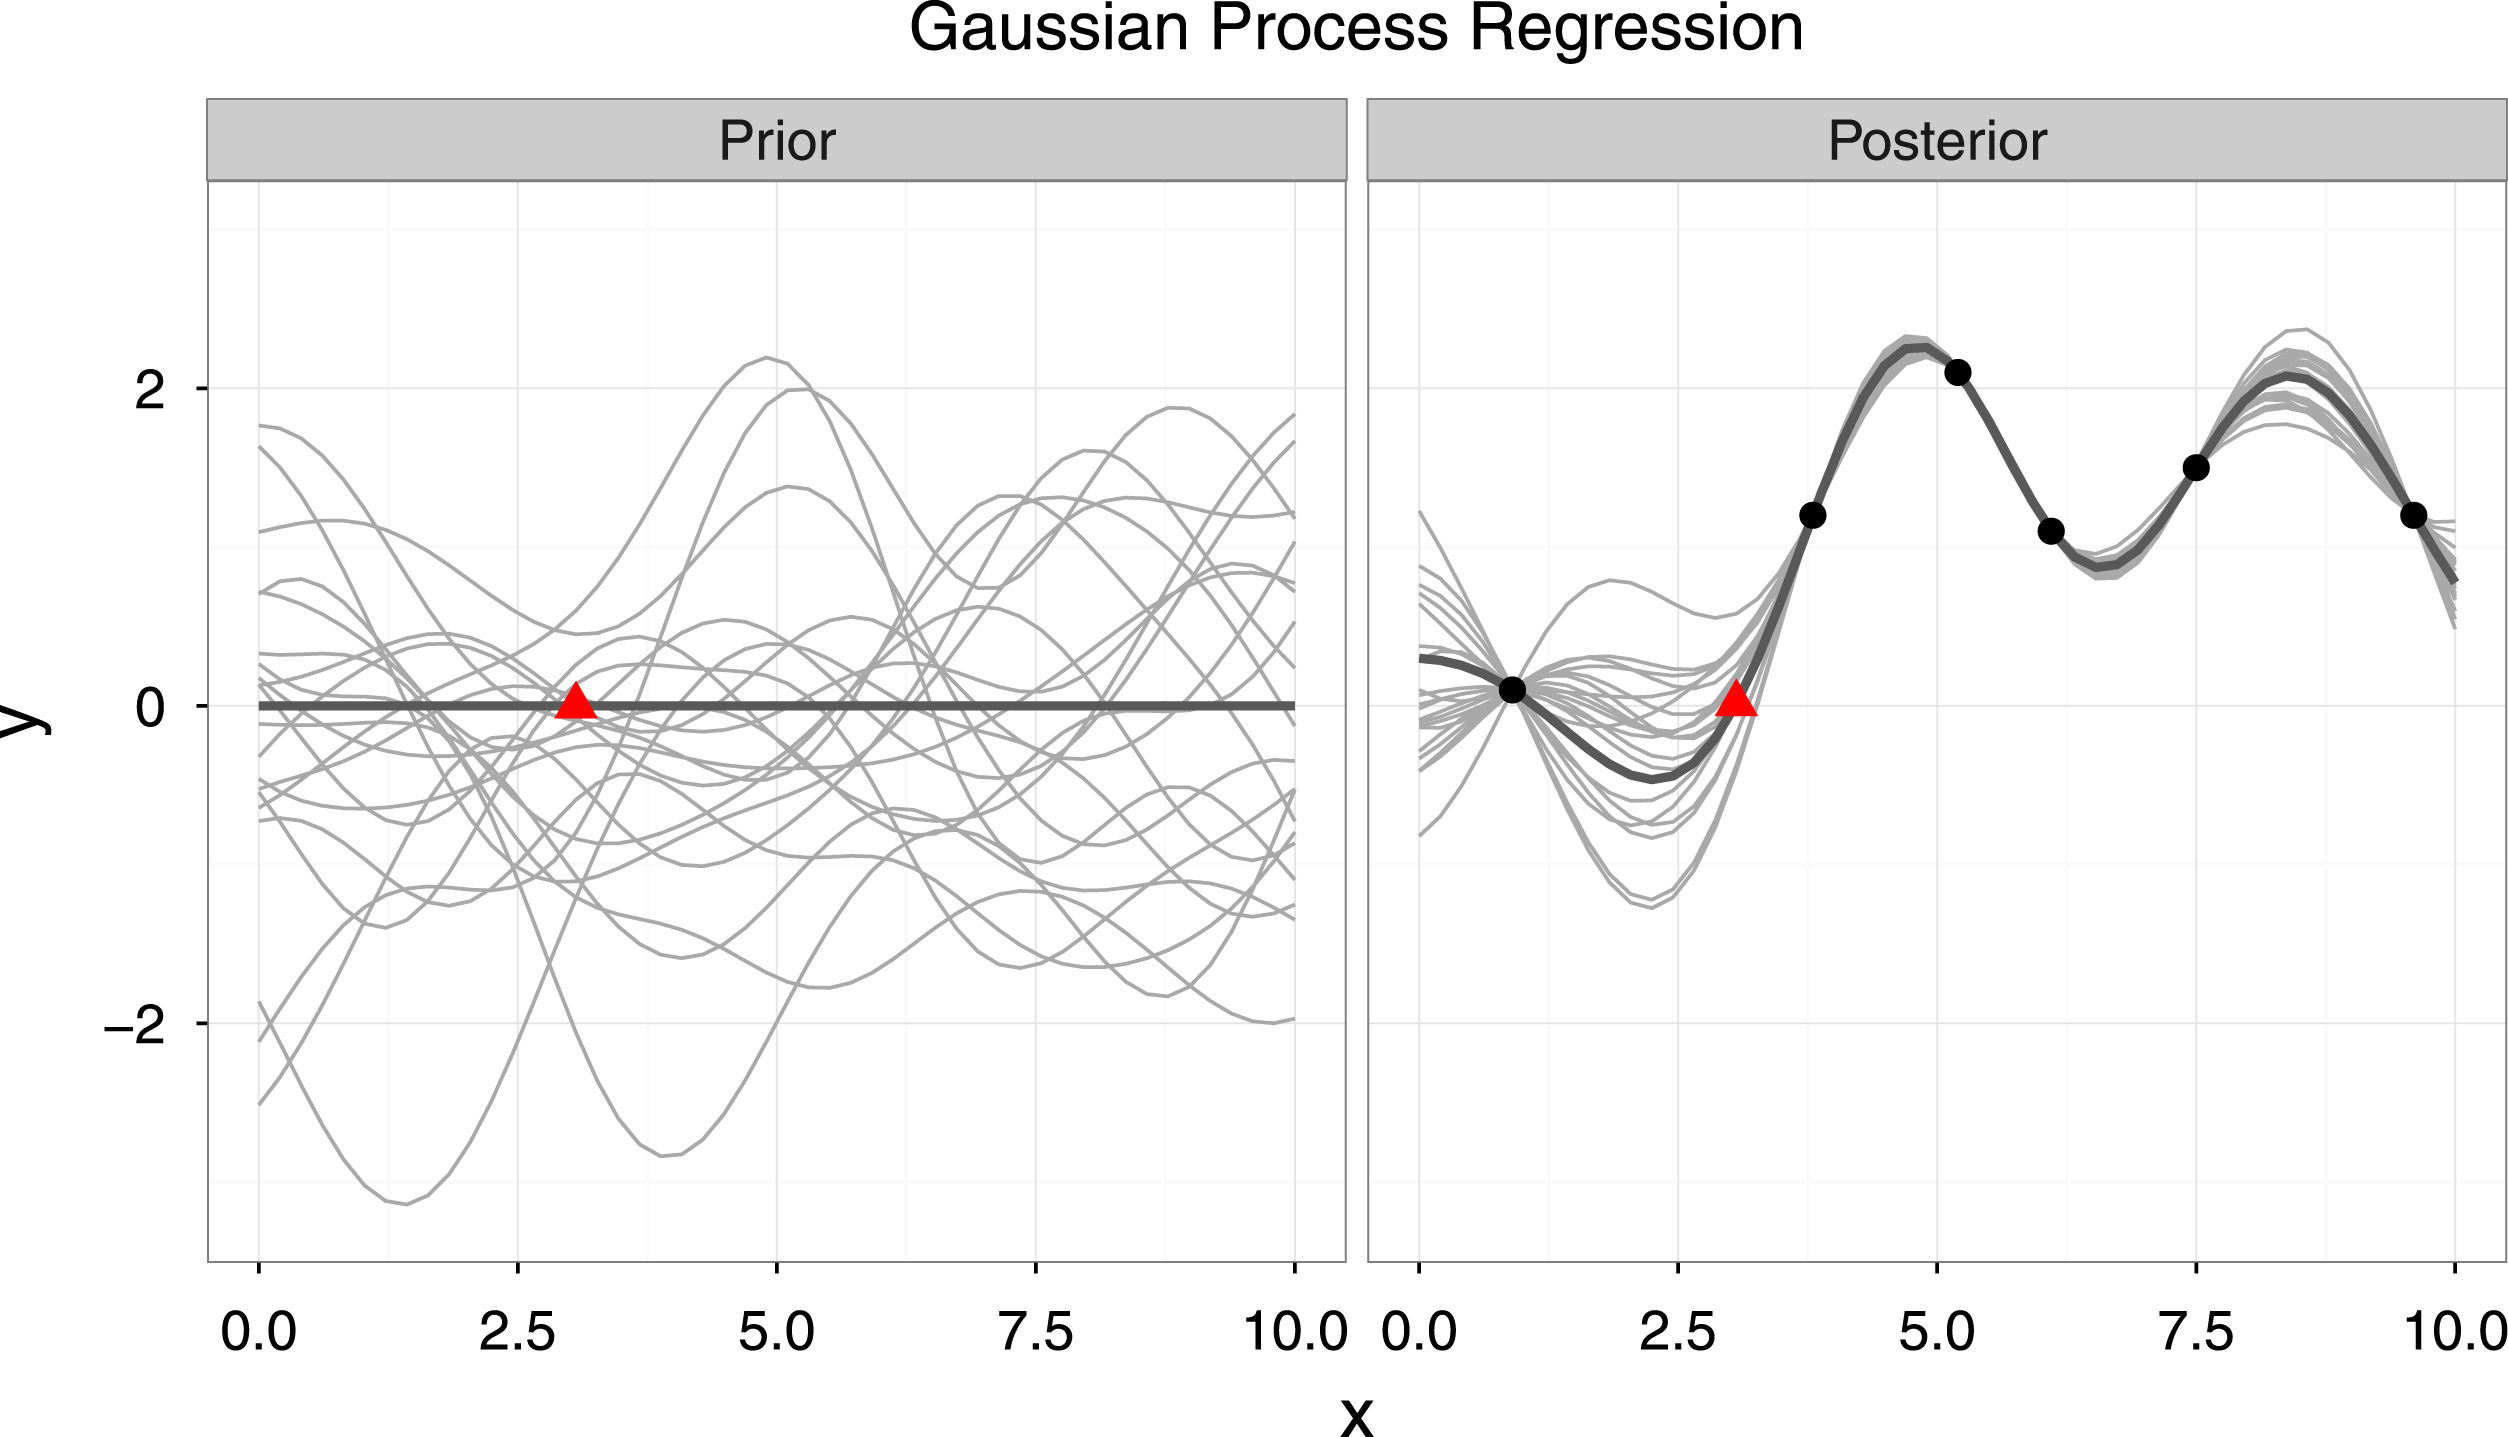
\includegraphics[height=0.50\textheight, trim = {195 7 0 10}, clip]{figs/gpr_example.jpg} % Plots from the above paper on AE
%		%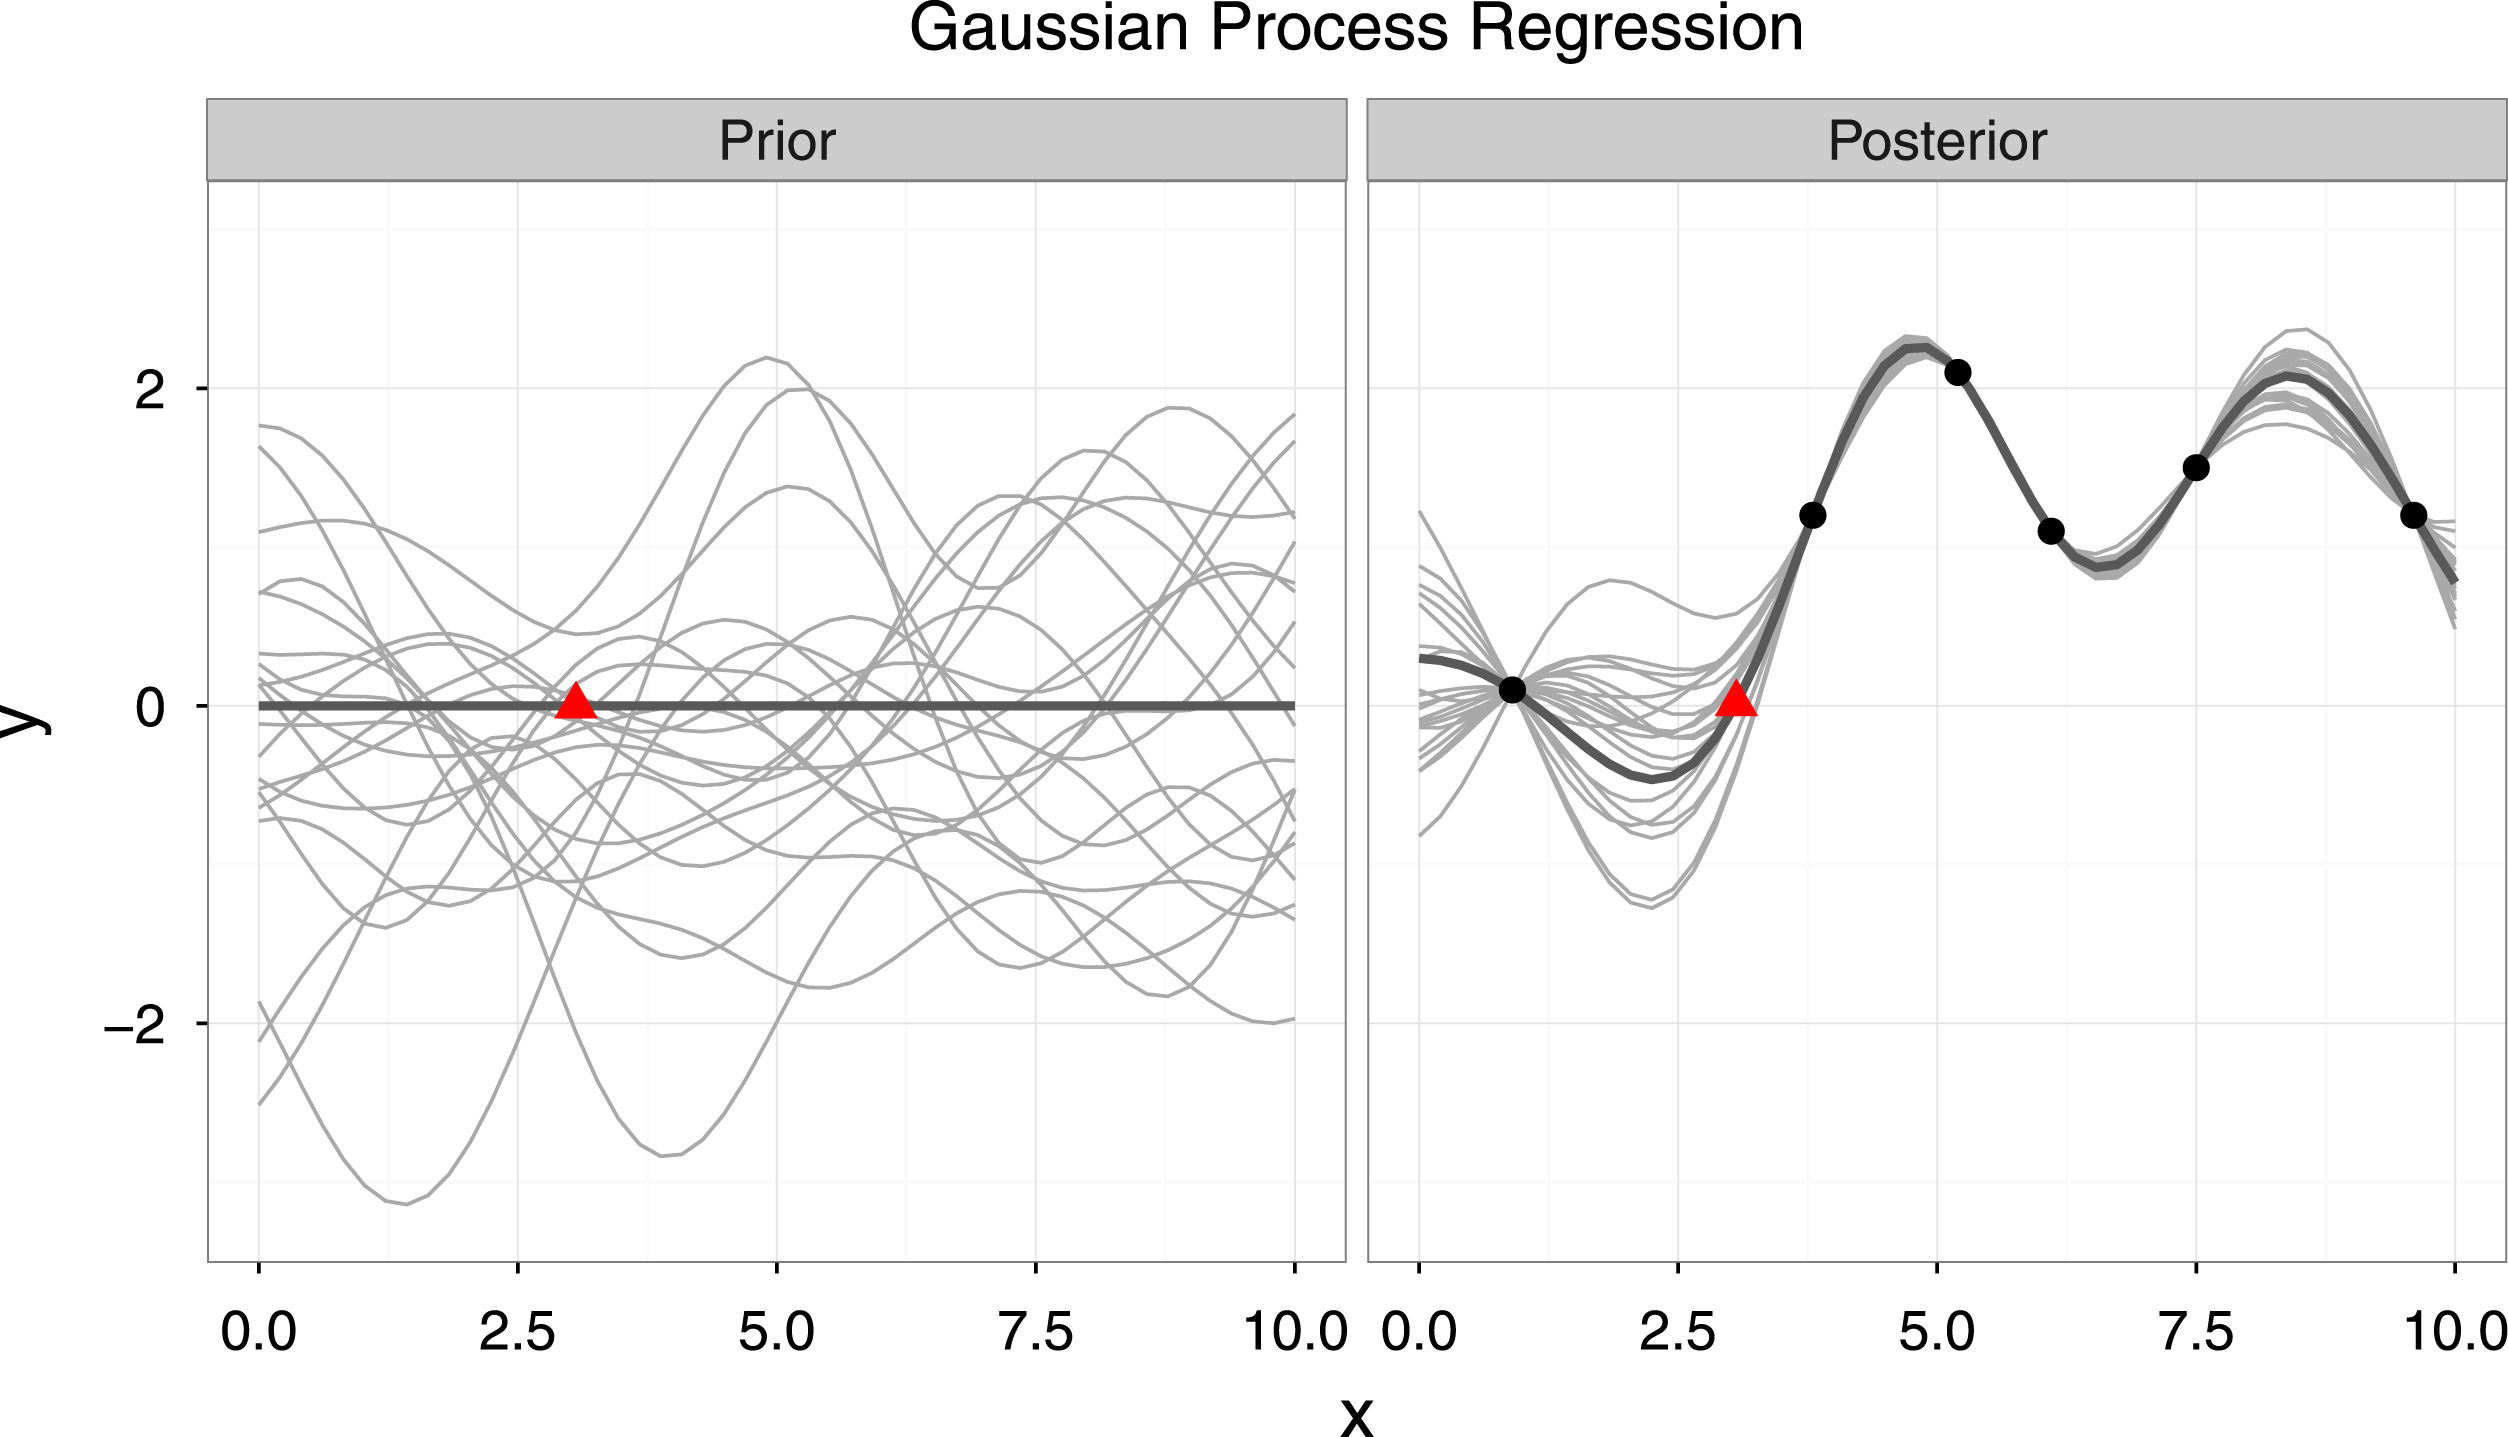
\includegraphics[height=0.40\textheight, trim = {198 70 2 40}, clip]{figs/gpr_example.jpg} % Plots from the above paper on AE
%	\end{figure}
%\end{frame}


\begin{frame}{Example: ``Active-learning and materials design: the example of high glass transition temperature polymers''}
	\begin{itemize}[label=\textbullet]
		\setlength{\itemsep}{0.6em}
		\item \textbf{Goal:} Find polymers with high glass transition temperature ($T_g$).
		\footnote{
			\tiny
			Kim, C., Chandrasekaran, A., Jha, A., \& Ramprasad, R. (2019). 
			Active-learning and materials design: The example of high glass transition temperature polymers. MRS Communications, 9(3), 860–866. 
			%https://doi.org/10.1557/mrc.2019.78
		}
		\item Glassy Temperature ($T_g$) is the temperature at which a polymer transitions from a hard, glassy state to a soft, rubbery state.
		\item Important for plastic materials used at high temperature.
	\end{itemize}
	\begin{figure}
		\centering
		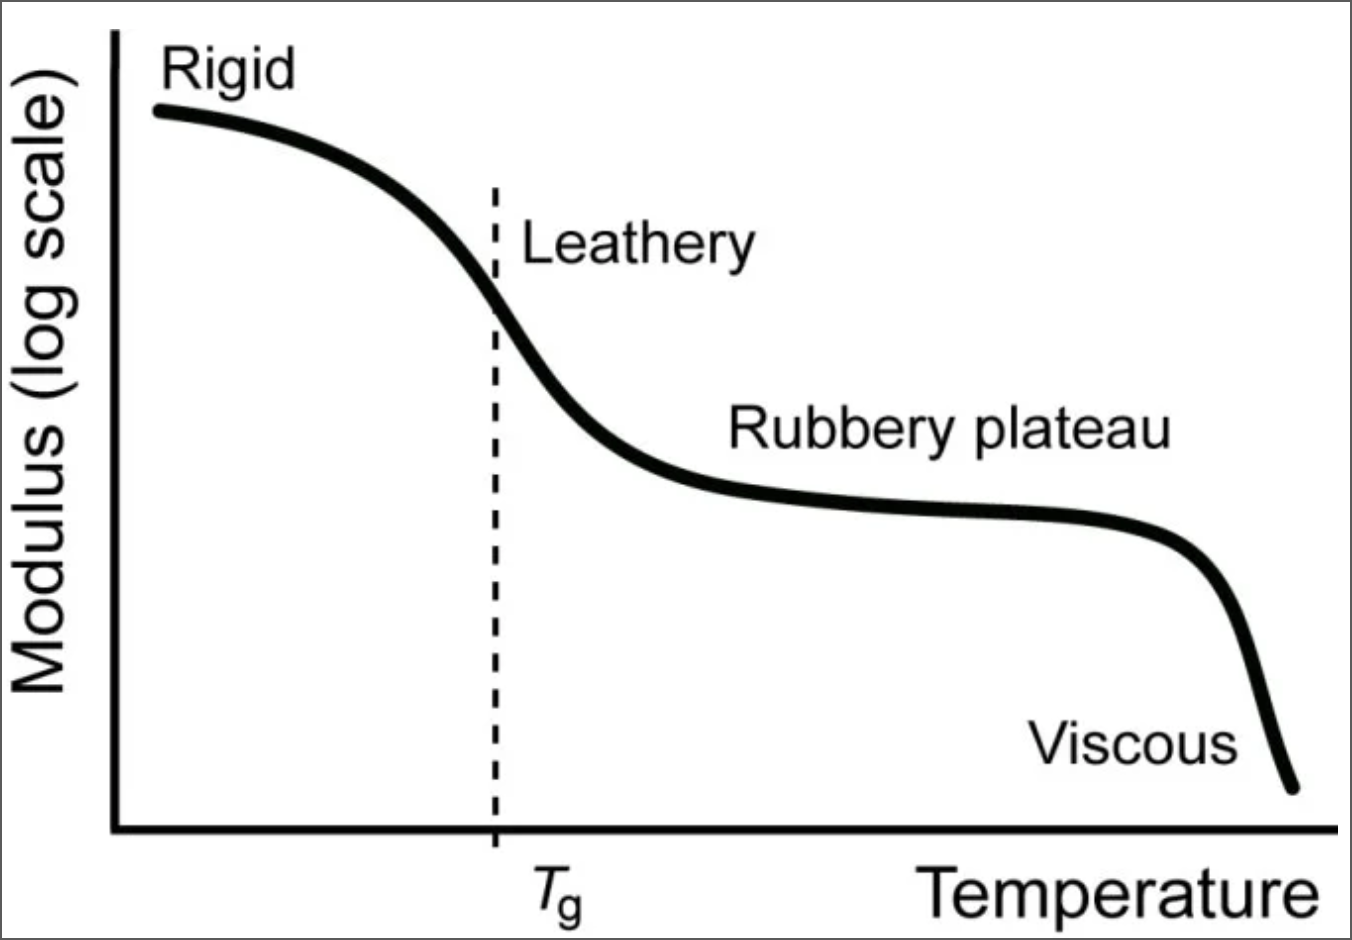
\includegraphics[height=0.35\textheight, trim = {4 4 4 4}, clip]{figs/glassy_transition.png} % Plots from the above paper on AE
	\end{figure}
\end{frame}

\begin{frame}{Dataset}
	\begin{itemize}[label=\textbullet]
		\setlength{\itemsep}{1.0em}
		\item \textbf{Dataset:} Online repository with $N = 736$ polymers.
		\item \textbf{Feature set:} $D = 244$ dimensional hierarchical polymer fingerprints.
			\vspace{0.5em}
			\begin{itemize}
			\setlength{\itemsep}{0.8em}
			
			\item \textbf{Atomic-scale descriptors (123 features):}
			%Count occurrences of specific atomic triples (three connected atoms, e.g., O–C–C) to capture local bonding environments and chemical composition.
			Occurrences of sets of 3 bonded atoms.
			
			\item \textbf{Molecular descriptors (99 features):}
			Quantitative structure-property descriptors, e.g. van der Waals surface area and fraction of rotatable bonds.
			
			\item \textbf{Morphological descriptors (22 features):}
			Larger-scale structural features, e.g. ring spacing and maximum side-chain length.
			\end{itemize}
	\end{itemize}
	\begin{figure}
		\centering
		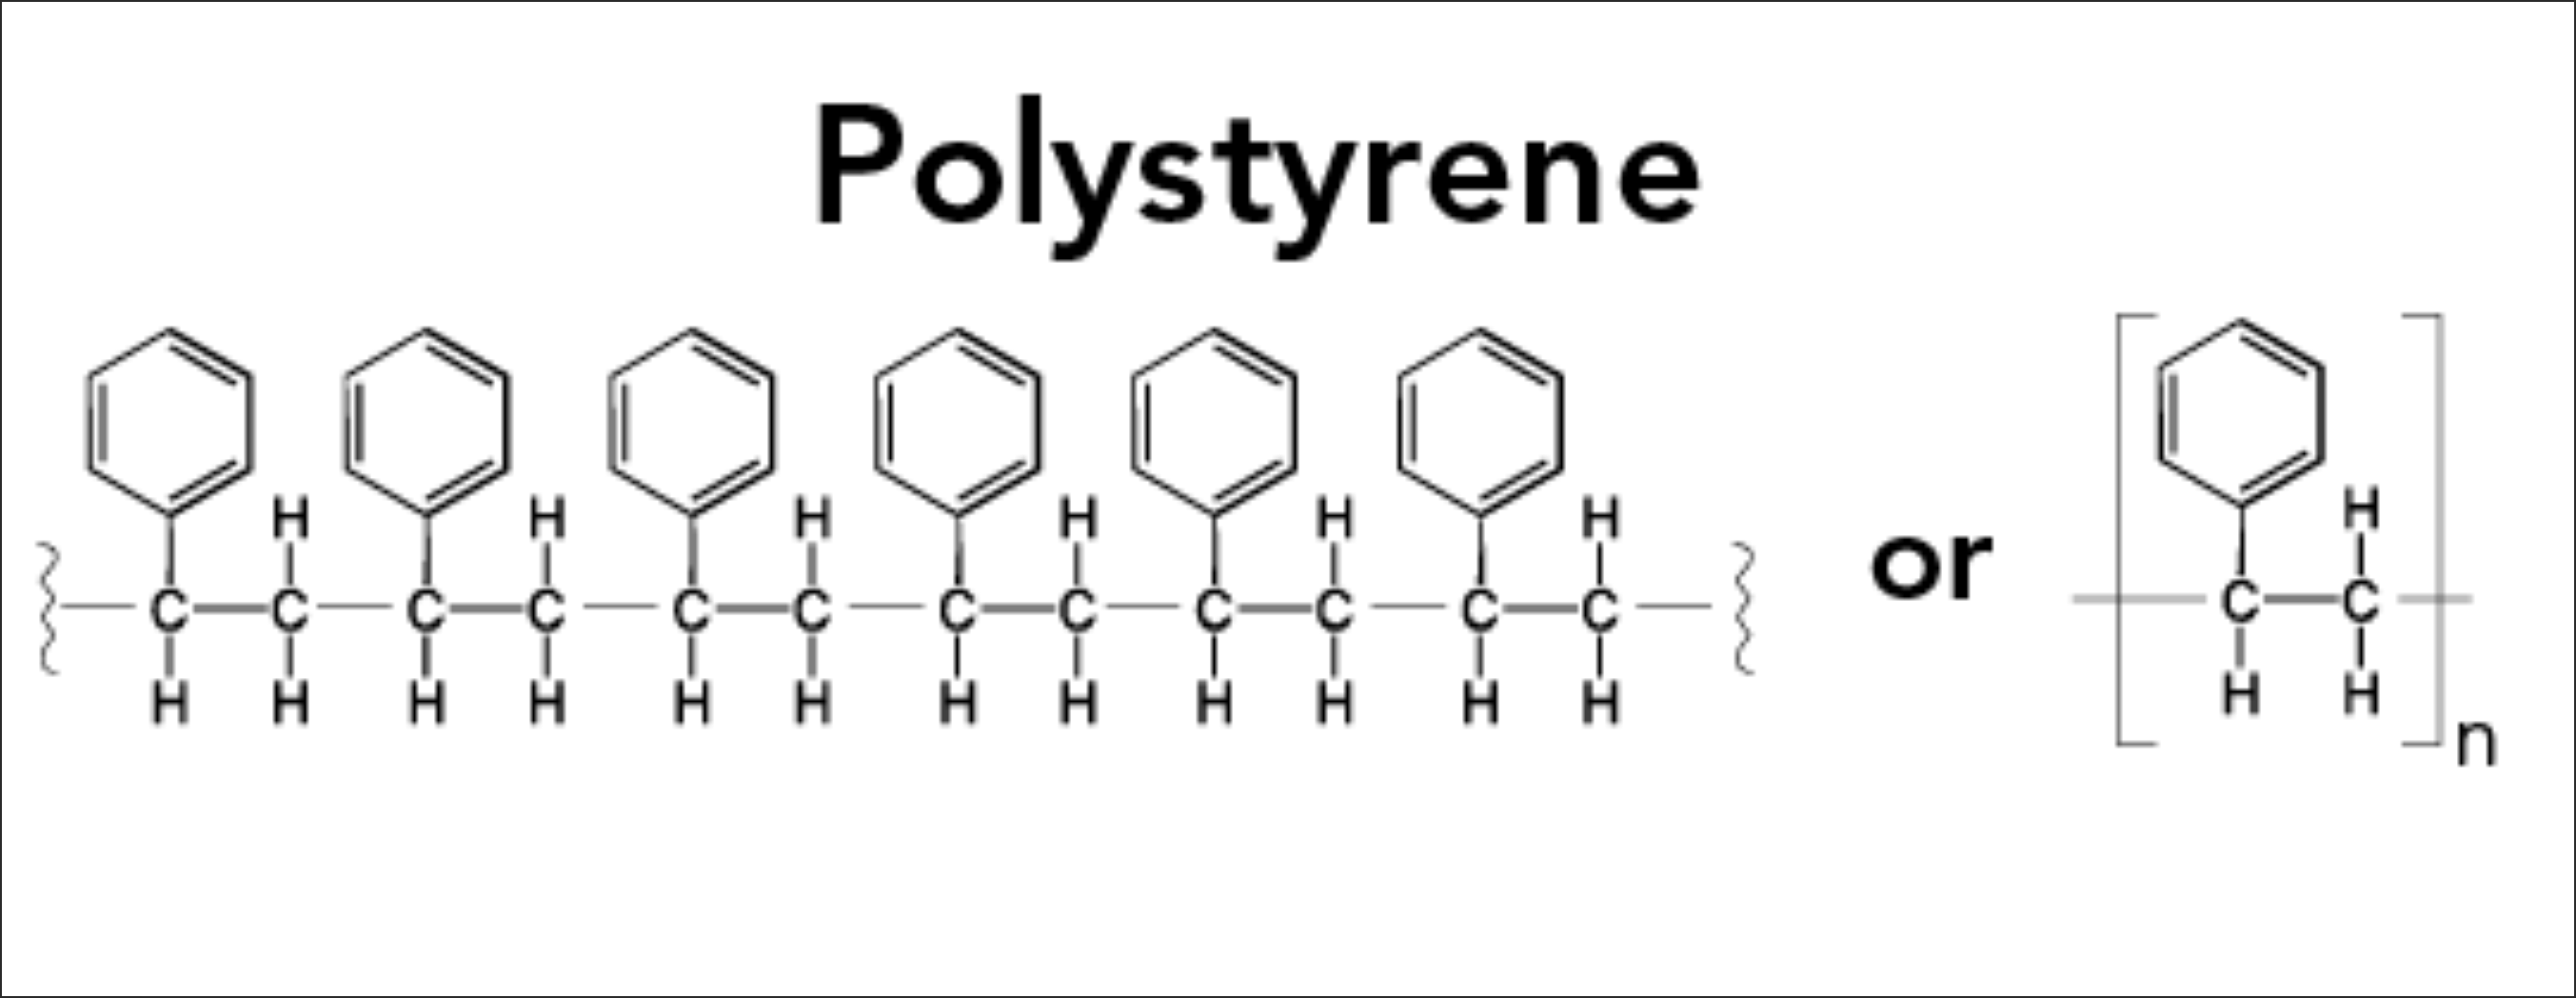
\includegraphics[height=0.20\textheight, trim = {4 200 800 300}, clip]{figs/polystyrene.png} % Plots from the above paper on AE
		\footnote{
			\tiny
			https://letstalkscience.ca/educational-resources/stem-explained/polystyrene-pros-cons-chemistry
		}
	\end{figure}
\end{frame}

\begin{frame}{Dataset Preprocessing}
	\begin{columns}[T]
		\column{0.75\textwidth}
		\begin{itemize}[label=\textbullet]
			\setlength{\itemsep}{1.6em}
			\item $D = 244 \to 2$ with principal component analysis (PCA).
			\item PCA: Uses correlation to reduce redundant dimensionality.
		\end{itemize}
		\vspace{2em}
		\begin{figure}
			\centering
			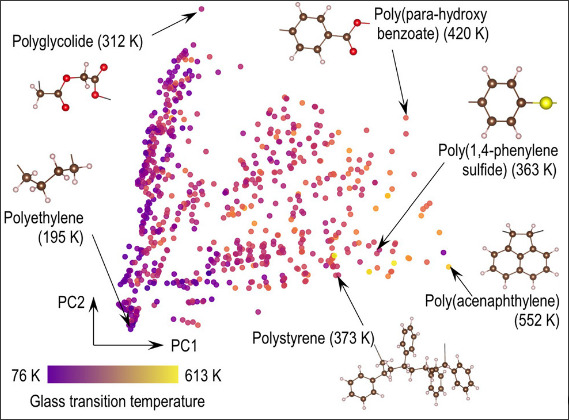
\includegraphics[height=0.50\textheight, trim = {2 2 2 2}, clip]{figs/exploration_vs_exploitation_figure0.png} % Plots from the above paper on AE
		\end{figure}
		\column{0.25\textwidth}
		\centering
		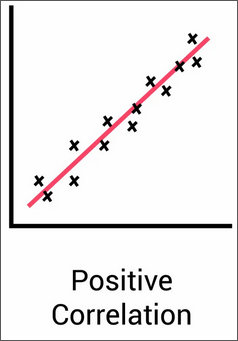
\includegraphics[width=0.7\linewidth, trim = {2 2 2 2}, clip]{figs/correlated.png} % Plots from the above paper on AE
		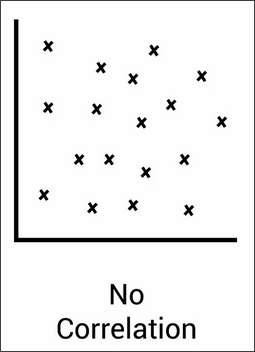
\includegraphics[width=0.7\linewidth, trim = {2 2 2 2}, clip]{figs/uncorrelated.png} % Plots from the above paper on AE
	\end{columns}
	\footnote{
		\tiny
		Figure from:
		Kim, C., Chandrasekaran, A., Jha, A., \& Ramprasad, R. (2019). 
		Active-learning and materials design: The example of high glass transition temperature polymers. MRS Communications, 9(3), 860–866. 
		%https://doi.org/10.1557/mrc.2019.78
	}
\end{frame}

\begin{frame}{Balanced Exploration--Exploitation Finds More High Tg Polymers}
	\begin{itemize}[label=\textbullet]
		\setlength{\itemsep}{0.6em}

		\item 4 Strategies compared to find $T_g > 450$ K.
		
		\item Best overall strategy: balanced exploration--exploitation.
		
		\item Achieves both \textbf{high mean performance} and \textbf{low variance}.
		
		\item Pure exploitation can perform well but is \textbf{sensitive to the initial dataset} and can get stuck in local optima.
		
	\end{itemize}
	
	\begin{figure}
		\centering
		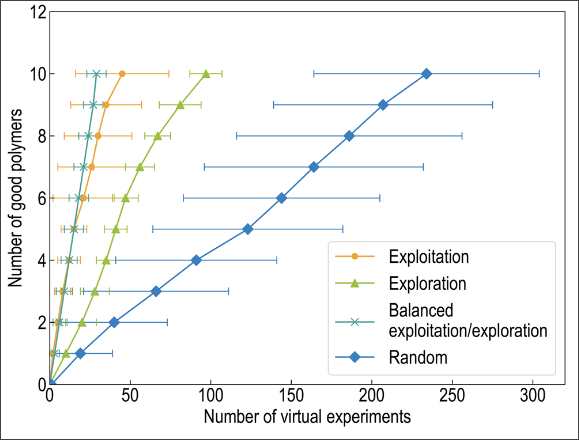
\includegraphics[height=0.45\textheight, trim = {2 2 2 2}, clip]{figs/exploration_vs_exploitation_figure.png}
	\end{figure}
\end{frame}


\begin{frame}{Balanced Strategies Discover Good Polymers Faster}

	\begin{columns}[T]
	
	\column{0.45\textwidth}
	
	\begin{itemize}[label=\textbullet]
	    \setlength{\itemsep}{3.6em}
		\vspace{1.5em}
	    \item Random search is the \textbf{least efficient} strategy.
	    
	    \item Exploitation performs well when the \textbf{initial dataset is large}.
	    
	    \item Balanced strategies perform best when the \textbf{search problem is difficult}.
	    
	\end{itemize}
	
	
	\column{0.55\textwidth}
	
	\begin{figure}
	    \centering
	    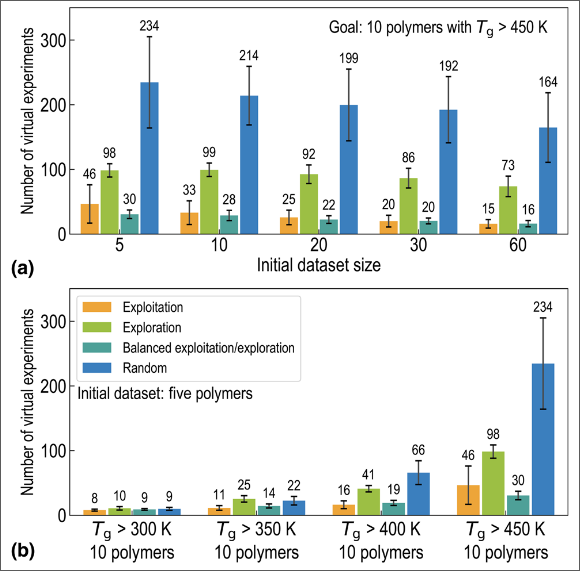
\includegraphics[width=\linewidth, trim = {4 4 4 4}, clip]{figs/fig5.png}
	\end{figure}
	
	\end{columns}

\end{frame}

\begin{frame}{Conclusion}
	\begin{itemize}[label=\textbullet]
	    \setlength{\itemsep}{1.6em}
		\item Gaussian Processes are a powerful tool for modeling unknown functions with uncertainty.
		\item Active Learning leverages this uncertainty to strategically select data points that improve the model.
		\item There is a rich ecosystem of acquisition functions that balance exploration and exploitation.
		\item We explored an example where acquisition functions were used for optimization but this framework can be applied to many other problems, e.g. learning a function globally.
	\end{itemize}
\end{frame}


\begin{frame}{Thank you}
  \Large \centering
  \vspace{2cm}
  \textbf{Thank you for your attention!}
  \vspace{1cm}

  And an extra thank you to Dr. Kreplak and the 207 office group for their help and feedback on this presentation.
\end{frame}


\begin{frame}{A Gaussian Process is a Distribution over Functions}
	\begin{itemize}
	    \setlength{\itemsep}{0.8em}
		\item A \textbf{multivariate Gaussian} describes a distribution over vectors:
		\[
		\mathbf{x} \sim \mathcal{N}(\boldsymbol{\mu}, \boldsymbol{\Sigma})
		\implies
		p(\mathbf{x})
		=
		\frac{1}{(2\pi)^{n/2} |\boldsymbol{\Sigma}|^{1/2}}
		\exp\!\left(
		-\frac{1}{2}
		(\mathbf{x}-\boldsymbol{\mu})^\top
		\boldsymbol{\Sigma}^{-1}
		(\mathbf{x}-\boldsymbol{\mu})
		\right).
		\]

		\item Depends on: the mean $\boldsymbol{\mu}$ and covariance matrix $\boldsymbol{\Sigma}$.

		\vspace{1.5em}
	
		\item A \textbf{Gaussian Process ($\mathcal{GP}$)} is the \emph{infinite-dimensional}
	    generalization of this idea. It describes a distribution over functions $f(x)$:
    	\[
			f(x) \sim \mathcal{GP}(m(x), k(x,x')).
    	\]

		\item Depends on: the mean function $m(x)$ and covariance function $k(x,x')$.

		\vspace{1.5em}

		\item \textbf{Key Idea}: Sampling $\mathcal{GP}$ at $\{x_1, x_2, \ldots, x_n\}$ gives a multivariate Gaussian distribution:
    	\[
			(f(x_1), f(x_2), \dots, f(x_n)) \sim \mathcal{N}(\boldsymbol{\mu}, \boldsymbol{\Sigma}).
    	\]
	\end{itemize}

	%\centering
	%\begin{tikzpicture}
	%
	%\node (img) at (0,0) {
	%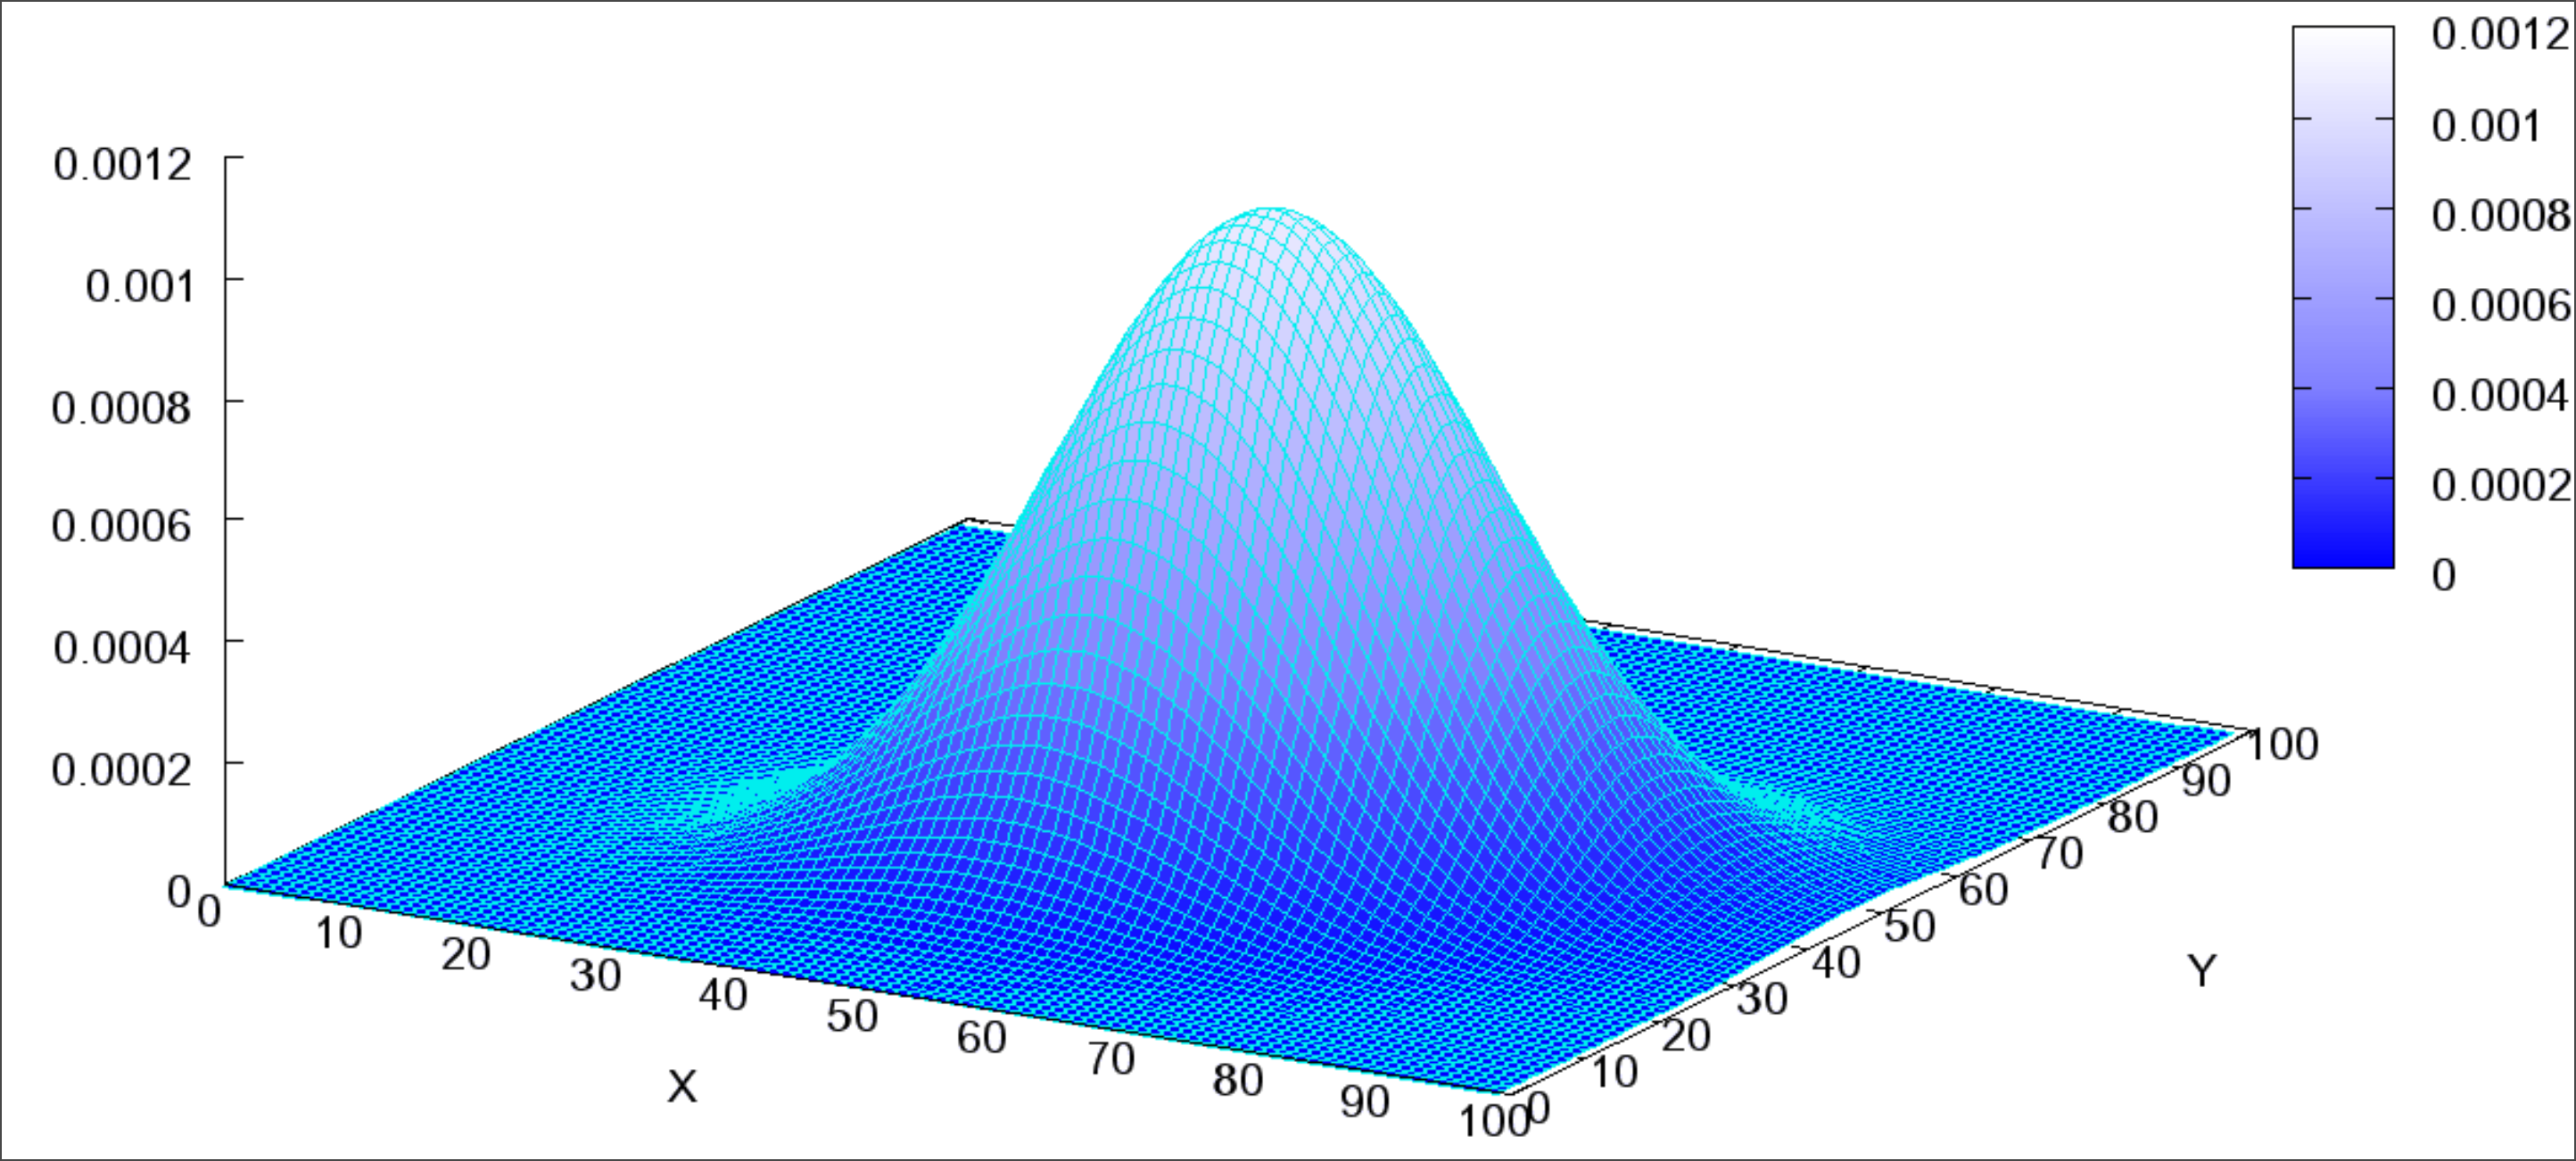
\includegraphics[
	%    width=0.4\textheight,
	%    trim=290 10 370 10,
	%    clip
	%]{figs/multivariate_normal.png}
	%};
	%
	%\node (arrow) at (3.0,0) {\Huge $\longrightarrow$};
	%
	%\node (inf) at (4.5,0) {\Huge $\infty$};
	%
	%\end{tikzpicture}

\end{frame}

\begin{frame}{Bayesian Linear Regression (Weight Space)}

\textbf{Model:}
\[
f(\mathbf{x}) = \mathbf{x}^\top \mathbf{w}
\]

\textbf{Data model (Gaussian noise):}
\[
y_i = \mathbf{x}_i^\top \mathbf{w} + \varepsilon_i,
\quad
\varepsilon_i \sim \mathcal{N}(0,\sigma_n^2)
\]

For a dataset with design matrix $X \in \mathbb{R}^{n\times d}$:

\textbf{Likelihood:}
\[
p(\mathbf{y}\mid X,\mathbf{w})
=
\prod_{i=1}^n \mathcal{N}(y_i \mid \mathbf{x}_i^\top \mathbf{w},\sigma_n^2)
=
\mathcal{N}(X\mathbf{w},\sigma_n^2 I)
\]

\textbf{Prior on weights:}
\[
\mathbf{w} \sim \mathcal{N}(\mathbf{0},\sigma_w^2 I)
\]

\textbf{Bayes' theorem gives a Gaussian posterior:}
\[
p(\mathbf{w}\mid X,\mathbf{y})
\propto
p(\mathbf{y}\mid X,\mathbf{w})p(\mathbf{w})
=
\mathcal{N}(\boldsymbol{\mu}_w,\boldsymbol{\Sigma}_w)
\]

\end{frame}

\begin{frame}{Prediction by Marginalizing the Weights}

Given a new input $\mathbf{x}_*$, we predict the latent output
\[
f_* = \mathbf{x}_*^\top \mathbf{w}.
\]

Because the weights are uncertain, we marginalize over their posterior:

\[
p(f_* \mid \mathbf{x}_*, X, \mathbf{y})
=
\int p(f_* \mid \mathbf{x}_*, \mathbf{w})
\, p(\mathbf{w}\mid X,\mathbf{y})\, d\mathbf{w}.
\]

\textbf{Predictive distribution:}
\[
p(f_* \mid \mathbf{x}_*, X, \mathbf{y})
=
\mathcal{N}(\mu_*,\sigma_*^2).
\]

\textbf{Why Gaussian?}
\begin{itemize}
\item The posterior $p(\mathbf{w}\mid X,\mathbf{y})$ is Gaussian.
\item The prediction $f_* = \mathbf{x}_*^\top \mathbf{w}$ is a linear function of $\mathbf{w}$.
\item A linear transformation of a Gaussian variable is Gaussian.
\end{itemize}

\textbf{Interpretation:}  
Bayesian regression places uncertainty on the weights and propagates this
uncertainty to predictions.

\end{frame}

\begin{frame}{Closed-Form Posterior and Predictive}

Recall:

\[
p(\mathbf{w}) = \mathcal{N}(\mathbf{0}, \sigma_w^2 I),
\qquad
p(\mathbf{y}\mid X,\mathbf{w}) = \mathcal{N}(X\mathbf{w}, \sigma_n^2 I).
\]

\textbf{Posterior over weights:}

\[
\boldsymbol{\Sigma}_w
=
\left(
\frac{1}{\sigma_n^2} X^\top X
+
\frac{1}{\sigma_w^2} I
\right)^{-1}
\]

\[
\boldsymbol{\mu}_w
=
\frac{1}{\sigma_n^2}
\boldsymbol{\Sigma}_w
X^\top \mathbf{y}
\]

\vspace{0.3cm}

\textbf{Predictive distribution at } $\mathbf{x}_*$:

\[
\mu_*
=
\mathbf{x}_*^\top \boldsymbol{\mu}_w
\]

\[
\sigma_*^2
=
\mathbf{x}_*^\top \boldsymbol{\Sigma}_w \mathbf{x}_*
+
\sigma_n^2
\]

\textbf{Interpretation:}
\begin{itemize}
\item Posterior mean = regularized least squares solution.
\item Predictive variance = model uncertainty + observation noise.
\end{itemize}

\end{frame}


\begin{frame}{Choosing a Good Basis for Infinite Feature Spaces}
	A naive polynomial feature map
	\[
	\boldsymbol{\phi}(x) = (1, x, x^2, \ldots)^\top
	\]
	induces the kernel
	\[
		k(x,x') = \sum_{n=0}^\infty x^n x'^n,
	\]
	This is problematic because:
	\begin{itemize}
		\item The kernel is \emph{not stationary} (depends on absolute position).
		\item The basis of the feature space is \emph{not orthogonal}.
		\item The series \emph{does not converge} for $|x x'| \geq 1$.
	\end{itemize}

	Using an orthogonal basis with a decaying envelope, e.g.
	\[
		\phi_n(x) = H_n(x)\,e^{-x^2/2}, 
	\]
	where $H_n(x)$ are Hermite polynomials.
	Then $\Sigma_w$ is diagonal with decaying entries, ensuring convergence of the kernel expansion.
\end{frame}

\begin{frame}{Projections into Feature Space (Theory)}
	Our previous model is limited to linear functions, but we can extend it to non-linear functions by projecting our inputs into a higher-dimensional \emph{feature space} using a mapping $\boldsymbol{\phi}(\mathbf{x})$. For example, 
	% row
	\[
		\boldsymbol{\phi}(\mathbf{x}) = (1, \mathbf{x}, \mathbf{x}^2, \ldots)^\top.
	\]

	Then our model becomes $f(\mathbf{x}) = \boldsymbol{\phi}(\mathbf{x})^\top \mathbf{w}$. Since everything is still linear in $\mathbf{w}$, all of our previous results still hold, we just need to replace $\mathbf{x}$ with $\boldsymbol{\phi}(\mathbf{x})$ everywhere so the predictive distribution is now normally distributed:
	$\mathcal{N}\!\left( \mu_*, \, \sigma_*^2 \right)$.
	\[
	\mu_* =
	\boldsymbol{\phi}(\mathbf{x}_*)^\top
	\Sigma_w
	\boldsymbol{\Phi}
	\left(
	\boldsymbol{\Phi}^\top \Sigma_w \boldsymbol{\Phi}
	+ \sigma_n^2 \mathbf{I}
	\right)^{-1}
	\mathbf{y},
	\]
	\[
	\sigma_*^2 =
	\boldsymbol{\phi}(\mathbf{x}_*)^\top
	\Sigma_w
	\boldsymbol{\phi}(\mathbf{x}_*)
	-
	\boldsymbol{\phi}(\mathbf{x}_*)^\top
	\Sigma_w
	\boldsymbol{\Phi}
	\left(
	\boldsymbol{\Phi}^\top \Sigma_w \boldsymbol{\Phi}
	+ \sigma_n^2 \mathbf{I}
	\right)^{-1}
	\boldsymbol{\Phi}^\top
	\Sigma_w
	\boldsymbol{\phi}(\mathbf{x}_*).
	\]

Then we define the kernel function as 
$k(\mathbf{x}, \mathbf{x}') = \boldsymbol{\phi}(\mathbf{x})^\top \Sigma_w \boldsymbol{\phi}(\mathbf{x}')$,
which allows us to rewrite the predictive mean and variance as
\[
	\mu_* =
	\mathbf{k}_*^\top
	\left( K + \sigma_n^2 \mathbf{I} \right)^{-1}
	\mathbf{y},
	\quad
	\sigma_*^2 =
	k(\mathbf{x}_*, \mathbf{x}_*)
	-
	\mathbf{k}_*^\top
	\left( K + \sigma_n^2 \mathbf{I} \right)^{-1}
	\mathbf{k}_*,
\]
\[
	\text{where }
	K_{ij} = k(\mathbf{x}_i, \mathbf{x}_j)
	\quad
	\mathbf{k}_* = [k(\mathbf{x}_*, \mathbf{x}_1), \ldots, k(\mathbf{x}_*, \mathbf{x}_n)]^\top
\]
\end{frame}

\begin{frame}{Gaussian Process Regression -- Math}
	\begin{itemize}
	\setlength{\itemsep}{1.4em}
	%\item We have a $\mathcal{GP}$ for our \emph{prior dataset} $X = \{\mathbf{x}_1, \ldots, \mathbf{x}_n\}$, $\mathbf{y} = \{y_1, \ldots, y_n\}$:
	\item Given the dataset $X = \{\mathbf{x}_1,\ldots,\mathbf{x}_n\}$, $\mathbf{y} = (y_1, \ldots, y_n)$, we have a $\mathcal{GP}$ prior
		\[
			\mathbf{y} \sim \mathcal{N}(\mathbf{0}, K(X,X)), \quad \text{where } \quad
			K(X,X) = \begin{pmatrix}
				k(\mathbf{x}_1, \mathbf{x}_1) & \cdots & k(\mathbf{x}_1, \mathbf{x}_n) \\
				\vdots & \ddots & \vdots \\
				k(\mathbf{x}_n, \mathbf{x}_1) & \cdots & k(\mathbf{x}_n, \mathbf{x}_n)
			\end{pmatrix} 
		\]
	%\item By definition of a $\mathcal{GP}$, the joint distribution of observed data and a new point $x_*$ is also Gaussian:
	\item Sampling a $\mathcal{GP}$ at $X$ and a new point $\mathbf{x}_*$ gives a \textbf{joint Gaussian}:
		\[
		\begin{bmatrix}
		\mathbf{y} \\
		f(\mathbf{x}_*)
		\end{bmatrix}
		\sim
		\mathcal{N}
		\left(
		\mathbf{0},
		\begin{bmatrix}
			K(X,X) & K(X,\mathbf{x}_*) \\
			K(\mathbf{x}_*,X) & K(\mathbf{x}_*,\mathbf{x}_*)
		\end{bmatrix}
		\right).
		\]
	\item Prediction are obtained by conditioning the joint Gaussian:
	\[
		p(f(\mathbf{x}_*) \mid \mathbf{x}_*, X,\mathbf{y}) = \mathcal{N}(\mu_*,\sigma_*^2).
	\]
	where $\mu_*$ and $\sigma_*^2$ are given by closed-form expressions in terms of the kernel.
	\end{itemize}
\end{frame}

\begin{frame}{Acquisition Function -- Expected Improvement (Theory)}

	\textbf{Expected Improvement (EI):} for the GP predictive distribution 
	$f(\mathbf{x}) \sim \mathcal{N}(\mu_n(\mathbf{x}), \sigma_n^2(\mathbf{x}))$
	relative to a threshold $\tau$ (e.g.\ the best observed value).
	\footnote{
	\tiny
	Shahriari et al. (2016). Taking the Human Out of the Loop: A Review of Bayesian Optimization.
	}
	
	Define the improvement random variable
	\[
	I(\mathbf{x}) = \max(0, f(\mathbf{x}) - \tau).
	\]
	
	The expected improvement is
	\begin{align*}
	\alpha_{\mathrm{EI}}(\mathbf{x})
	&= \mathbb{E}[I(\mathbf{x})] \\
	&= \int_\tau^\infty (f - \tau) \mathcal{N}(f \mid \mu_n(\mathbf{x}), \sigma_n^2(\mathbf{x})) df \\
	&= \int_\tau^\infty (f - \tau) \frac{1}{\sqrt{2\pi}\sigma_n(\mathbf{x})} \exp\!\left(-\frac{(f - \mu_n(\mathbf{x}))^2}{2\sigma_n^2(\mathbf{x})}\right) df \\
	&= (\mu_n(\mathbf{x}) - \tau) \Phi(z) + \sigma_n(\mathbf{x}) \phi(z),\quad
	z = \frac{\mu_n(\mathbf{x}) - \tau}{\sigma_n(\mathbf{x})}
	\end{align*}
	and $\Phi$ and $\phi$ are the CDF and PDF of the standard normal distribution.	The LHS term is large when the mean is much better than the threshold, and the RHS term is large when there is high uncertainty.
\end{frame}
\begin{frame}{Acquisition Function -- Information Gain (Theory)}
	\textbf{Information Gain (IG):} how much we expect our uncertainty about $f$ to decrease by sampling at $\mathbf{x}$:
	\begin{align*}
		\alpha_{\mathrm{IG}}(\mathbf{x})
		&= H\!\left[p(f \mid \mathcal{D})\right] - \mathbb{E}_{y \sim p(y \mid \mathbf{x}, \mathcal{D})}\!\left[H\!\left[p(f \mid \mathcal{D} \cup \{(\mathbf{x}, y)\}\right]\right].
	\end{align*}
	\textbf{Prior Entropy:} 
	\[
		H\!\left[p(f \mid \mathcal{D})\right] = -\int p(f \mid \mathcal{D}) \log p(f \mid \mathcal{D}) \, df
	\]
	\[
		= -\int \mathcal{N}(f \mid \mu_n(\mathbf{x}), \sigma_n^2(\mathbf{x}))
		\log \mathcal{N}(f \mid \mu_n(\mathbf{x}), \sigma_n^2(\mathbf{x})) \, df
		= \frac{1}{2} \log\!\bigl(2\pi e\,\sigma_n^2(\mathbf{x})\bigr).
	\]
	\textbf{Posterior Entropy:} after observing a new point, the entropy has the same form but with the updated posterior variance:
	\[
		H\!\left[p(f \mid \mathcal{D} \cup \{(\mathbf{x}, y)\})\right]
		= \frac{1}{2} \log\!\bigl(2\pi e\,\sigma_{n+1}^2(\mathbf{x})\bigr).
	\]
	Therefore,
	\[
		\alpha_{\mathrm{IG}}(\mathbf{x})
		= \frac{1}{2}\log\!\bigl(2\pi e\,\sigma_n^2(\mathbf{x})\bigr)
		- \frac{1}{2}\log\!\bigl(2\pi e\,\sigma_{n+1}^2(\mathbf{x})\bigr)
		= \frac{1}{2}\log\!\left(\frac{\sigma_n^2(\mathbf{x})}{\sigma_{n+1}^2(\mathbf{x})}\right).
	\]
\end{frame}

\begin{frame}{Gaussian Process Regression (Hyperparameters)}
	\begin{itemize}[label=\textbullet]
		\setlength{\itemsep}{0.6em}
		\item The standard kernel for GPs is the RBF (squared exponential) kernel:
		\[
			k(\mathbf{x}, \mathbf{x}') = \sigma_f^2 \exp\left(-\frac{\|\mathbf{x} - \mathbf{x}'\|^2}{2\ell^2}\right),
		\]
	\end{itemize}
	\begin{figure}
		\centering
		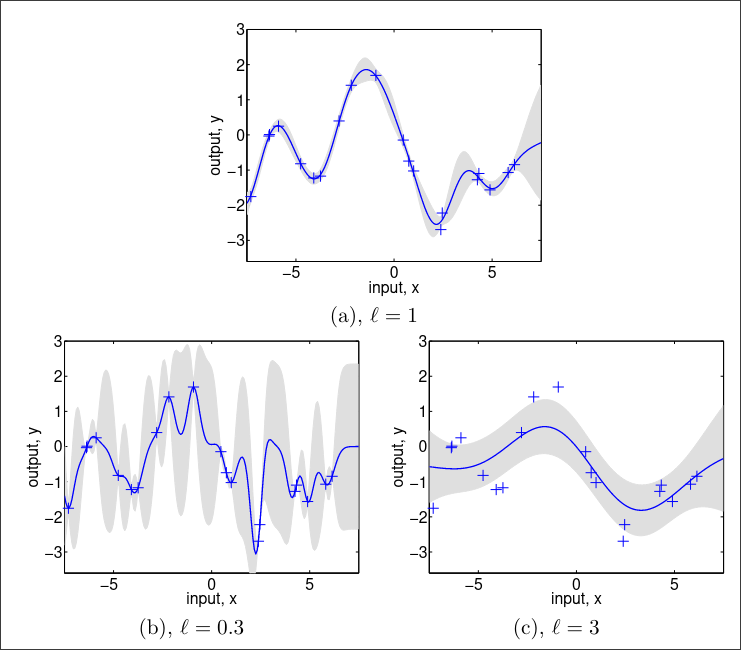
\includegraphics[width=0.6\linewidth]{figs/hyperparameter.png}
		%\caption{Example of GP regression with different hyperparameters.} %\footnote{https://www.lancaster.ac.uk/stor-i-student-sites/thomas-newman/2022/05/05/gaussian-processes-in-regression/}.
	\end{figure}
\end{frame}

\begin{frame}{Example: Thin Film Pseudomobility with Automated Experimentation}
	\begin{itemize}[label=\textbullet]
		\setlength{\itemsep}{0.6em}
		\item Example of using active learning to optimize the pseudomobility of a thin film.
			\footnote{
				\tiny
				MacLeod, B. P., et al. (2020). Self-driving laboratory for accelerated discovery of thin-film materials. Science Advances, 6(20), eaaz8867. 
				%https://doi.org/10.1126/sciadv.aaz8867
			}
	\end{itemize}
	\begin{figure}
		\centering
		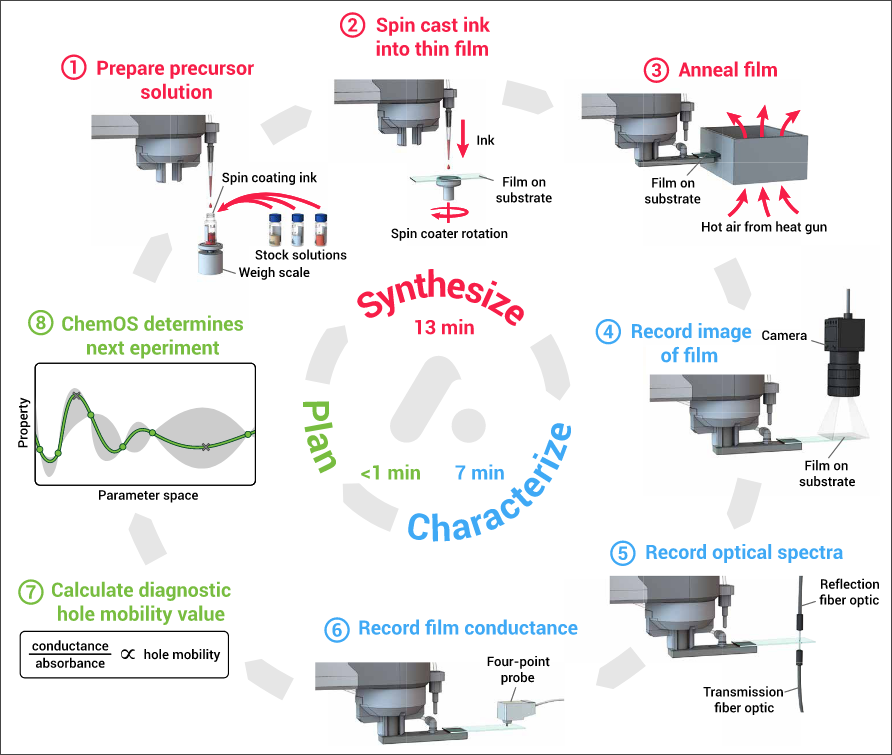
\includegraphics[width=0.6\linewidth, trim = {2 2 2 2}, clip]{figs/active_learning1.png} % Example of a AE (automated experimentation) loop
	\end{figure}
\end{frame}

\begin{frame}{Example: Thin Film Pseudomobility (Results)}
	\begin{itemize}[label=\textbullet]
		\setlength{\itemsep}{0.6em}
		\item This just looked for the minimum of a 2D function.
		\item Example of the strategy called \textbf{Expected Improvement}.
		\item Parameters: Dopant concentration and annealing time.
		\item Output: Pseudomobility of the thin film.
	\end{itemize}
	\begin{figure}
		\centering
		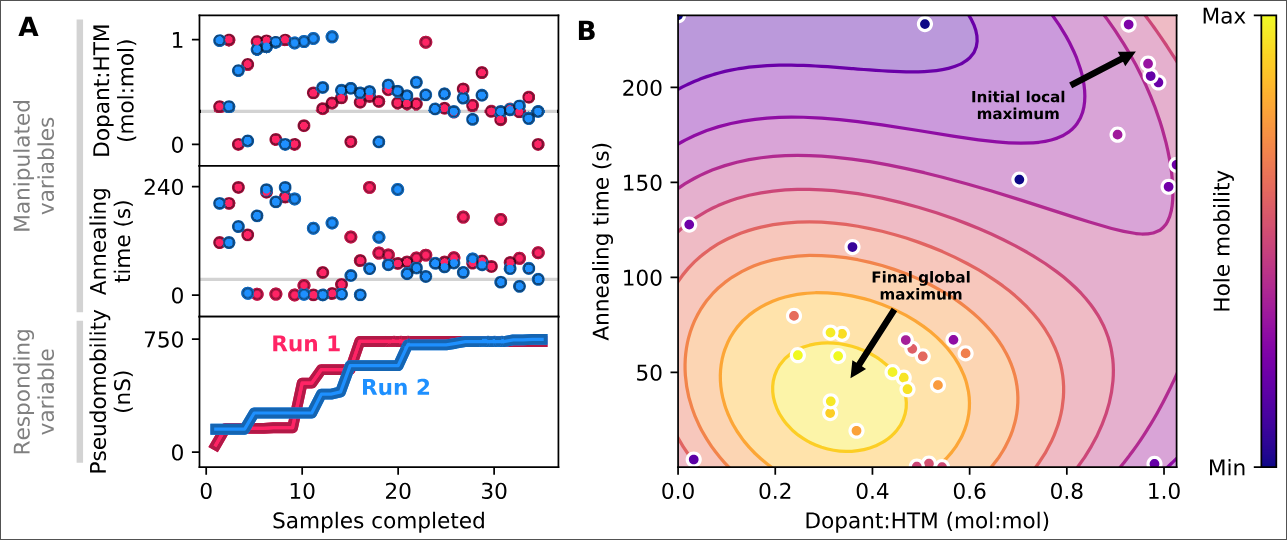
\includegraphics[width=0.9\linewidth, trim = {2 2 2 2}, clip]{figs/example1b.png} % Plots from the above paper on AE
	\end{figure}
\end{frame}

\begin{frame}{Hierarchical Polymer Fingerprints: Atomic Descriptors}

\begin{itemize}
\setlength{\itemsep}{1em}

\item \textbf{Local chemical environments} are captured using \textbf{atomic triples}.

\item An atomic triple is a sequence of three bonded atoms.

\[
\text{Example: } O{-}C{-}C
\]

\item Each atom is labeled by its \textbf{coordination number}
(number of bonds).

\[
C_4{-}C_3{-}O_2
\]

\item The fingerprint records how often each triple occurs in the
polymer repeat unit.

\item For this dataset there are \textbf{123 possible triples}.

\end{itemize}

\vspace{0.5em}

\textbf{Purpose:} capture the \textbf{local bonding chemistry}
that influences stiffness and chain mobility.

\end{frame}

\begin{frame}{Hierarchical Polymer Fingerprints: Molecular Descriptors}

\begin{itemize}
\setlength{\itemsep}{1em}

\item Quantitative structure-property descriptors are computed
from the molecular structure.

\item Examples include:

\begin{itemize}
\item \textbf{van der Waals surface area}
\item \textbf{Topological surface area}
\item \textbf{Fraction of rotatable bonds}
\end{itemize}

\item These descriptors capture global molecular properties that
affect polymer flexibility and packing.

\item All descriptors are computed using the
\textbf{RDKit cheminformatics library}.

\item This level contributes \textbf{99 features} to the fingerprint.

\end{itemize}

\vspace{0.5em}

\textbf{Purpose:} capture physical properties that influence
chain mobility and intermolecular interactions.

\end{frame}

\begin{frame}{Hierarchical Polymer Fingerprints: Morphological Descriptors}

\begin{itemize}
\setlength{\itemsep}{1em}

\item The third level captures \textbf{larger-scale structural features}
of the polymer.

\item Examples include:

\begin{itemize}
\item Topological distance between rings
\item Fraction of atoms in side chains
\item Length of the largest side chain
\end{itemize}

\item These descriptors characterize the \textbf{overall architecture}
of the polymer chain.

\item Structural morphology strongly influences
\textbf{packing, rigidity, and glass transition temperature}.

\item This level contributes \textbf{22 morphological descriptors}.

\end{itemize}

\vspace{0.5em}

\textbf{Purpose:} capture how the polymer structure extends
beyond local chemical bonds.

\end{frame}


\begin{frame}{Infinite Feature Maps are Not a Problem}
	\begin{itemize}
	\setlength{\itemsep}{2.0em}
	
	\item Recall: $\mathcal{GP}$ given by \textbf{mean} and \textbf{covariance} function.
	
	\item The \textbf{mean function} is\footnote{Prior: $\mathbf{w} \sim \mathcal{N}(\mathbf{0}, \sigma_w^2I)$}:
	\[
	m(x) = \mathbb{E}[f(x)]
		= \boldsymbol{\phi}(x)^\top \mathbb{E}[\mathbf{w}] = 0,
	\]
	
	
	\item The \textbf{covariance function} contains \emph{all of the information}:
	\[
	k(x,x')
	= \mathbb{E}\!\left[f(x)f(x')\right]
	= \boldsymbol{\phi}(x)^\top \mathbb{E}[\mathbf{w}\mathbf{w}^\top]
	\boldsymbol{\phi}(x')
	= \sigma_w^2 \boldsymbol{\phi}(x)^\top \boldsymbol{\phi}(x').
	\]
	
	\item We DO NOT need to compute the weights, but we DO need to compute large inner products.
	
	\end{itemize}
\end{frame}


\begin{frame}{The Kernel Trick}
	\begin{itemize}
	\setlength{\itemsep}{1.2em}
	
	\item Chose a specific feature map (there are other options):
	\[
	\boldsymbol{\phi}(x) =
	\left(
	1,\,
	x,\,
	\frac{x^2}{\sqrt{2!}},\,
	\frac{x^3}{\sqrt{3!}},\,
	\ldots
	\right).
	\]
	
	\item The kernel becomes
	
	\[
	k(x,x') =
	\boldsymbol{\phi}(x)^\top \boldsymbol{\phi}(x')
	=
	\sum_{n=0}^{\infty} \frac{(x x')^n}{n!}.
	\]
	
	\item This is the Taylor expansion of the exponential function:
	
	\[
	k(x,x') = e^{x x'}.
	\]
	
	\item Simple to compute but retains complexity.
	
	\end{itemize}
\end{frame}


\end{document}
